\chapter{Fianchetto: Accelerating Data Motion Across the Board}
\label{fianchetto:chap}

\newcommand{\arch}[0]{DRX\xspace}
\newcommand{\systemName}[0]{\emph{Fianchetto}\xspace}
\newcommand{\drx}[0]{DRX\xspace}
\newcommand{\drxs}[0]{DRXs\xspace}
\newcommand{\bench}[1]{{\textsf{#1}}\xspace}

\newcommand{\vs}[0]{\textsf{Video Surveillance}\xspace}
\newcommand{\sd}[0]{\textsf{Sound Detection}\xspace}
\newcommand{\bs}[0]{\textsf{Brain Stimulation}\xspace}
\newcommand{\pir}[0]{\textsf{Personal Info Redaction}\xspace}
\newcommand{\dhj}[0]{\textsf{Database Hash Join}\xspace}

% \section{Introduction}
% \label{fianchetto:sec:intro}
%\vspace{-2ex}

With the effective end of Dennard Scaling~\cite{dennard_scaling}, the dark silicon~\cite{dark_silicon_isca2011, dark_silicon:babak} phenomenon has led to the development and adoption of Domain-Specific Architectures (DSA) or accelerators.
%
With the Cambrian explosion of accelerators~\cite{diannao:asplos:2014, dnnoptimizing:fpga:2015, pudiannao:asplos:2015, shidiannao:isca:2015, cambricon:isca:2016, cambricon-x:micro:2016, cbrain:dac:2016, dnnweaver:micro:2016, fusedlayercnn:micro:2016, tabla:hpca:2016, escher:fccm:2017, pipelayer:hpca:2017, scnn:isca:2017, tpu:isca:2017, yongming-isca17, maeri:asplos18, unpu:isscc:2018, eyerissv2:journal:2019, simba:micro:2019, tangram:asplos19, awb-gcn:micro:2020, hygcn:hpca:2020,planaria:micro:2020, sigma:hpca:2020, engn:toc:2021, gcnax:hpca:2021, graphicionado:micro:2016, extrav:pvldb:2017, accugraph:pact:2018, hats:micro:2018, graphp:hpca:2018, graphr:hpca:2018, minnow:asplos:2018, conda:isca:2019, phi:micro:2019, graphpulse:micro:2020, deepgraph:hpca:2021, jetstream:micro:2021, lccg:sc:2021, darwin:asplos:2018, genax:isca:2018, smem:fpl:2018, asap:toc:2019, gencache:micro:2019, medal:micro:2019, genasm:micro:2020, geniehd:date:2020, nest:iccad:2020, savi:iccad:2020, seedex:micro:2020, wfa:fpl:2021, genstore:asplos:2022, segram:isca:2022, meet-the-walker:micro:2013,murray:micro:2016,robox:isca:2018,pointacc:micro:2021,robomorphic:asplos:2021}, it is fitting to consider the current cadence of the architecture design as the golden age of accelerators.  
%
Amazon Web Service (AWS)~\cite{aws-inferentia:2019, aws-trainium:2022}, Microsoft Azure~\cite{catapult:isca:2014, cloud-scale-acc:micro:2016, brainwave:isca:2018, microsoft-azure:zipline:2019}, and Google Cloud Platform (GCP)~\cite{tpu:isca:2017,tpuv4i:isca:2021,google-vcu:asplos:2021} as the three providers of public cloud recently started offering accelerator equipped instances. 
%

The offering of accelerator equipped instances is the result of market push toward hardware-accelerated compute-intensive applications such as genomics, content streaming, recommendation systems, virtual reality, data analytics, etc. 
%
Such applications often cross the boundary of multiple domains, each of which can be potentially accelerated with its own domain-specific architecture (DSA). 
%
These applications would maximally benefit from the DSAs in the cloud only if all the domains are accelerated and not just one. 
%

%
\begin{figure}[ht!]
    \centering
    \begin{subfigure}[b]{\columnwidth}
    \includegraphics[width=\textwidth]{figure/fianchetto/cpu-overview.pdf}
    \caption{Current multi-accelerator systems.}
    \label{fig:overview:current}
    \end{subfigure}
    %
    \hspace{0.5in}
    \begin{subfigure}[b]{\columnwidth}
    \includegraphics[width=\textwidth]{figure/fianchetto/dmx-overview.pdf}
    \caption{Multi-accelerator systems with \dmx.}
    \label{fig:overview:dmx}
    \end{subfigure}
    %
    \caption{Current multi-acceleration systems rely on CPU for accelerator chaining. (a) shows a system with four heterogeneous accelerator cards. The CPU needs to intervene in the communication between accelerator cards. This involves data copies from system memory to accelerator memory and non-trivial data transformations. (b) The proposed \dmx framework removes the CPU from the data path of multi-acceleration. \dmx delivers the performance of a monolithic accelerator while offering the composability and programmablity of the baseline system.}
    
\label{fig:overview}
\end{figure}

To enable heterogeneous cross-domain multi-acceleration, there is an essential need for cross-stack solutions for accelerator chaining to enable intimate communication between different DSAs, each of which is responsible for accelerating a part of a single application. 
%
This chapter sets out to explore a heterogeneous cross-domain multi-acceleration datacenter that harvests the recent initiative towards democratizing hardware design and enables the vision of a \textit{sea of accelerators}
~\cite{pymtl3:ieee-micro:2020, basejump:dac:2018, blackparrot:ieee-micro:2020, democratizing:cacm:2022, profiling:isca:2023}.

In a cross-domain multi-acceleration system, a chain of DSAs is created, where each DSA accepts inputs in a specific data structure and produces outputs in another data structure. 
%
The accelerator chaining currently needs to involve the system CPU (Figure~\ref{fig:overview}(a)) for restructuring and then exchanging data between different DSAs to run a single application.
%
This restructuring usually involves reshaping and reformatting the output of one DSA to match the input of the next.
%

We refer to the data restructuring and communication overhead of executing a single application using a number of different DSA as \textit{data motion} overhead. % in multi-accelerator systems.
%
Using the CPU for data motion requires frequent copies between the host and the DSA memory. 
%
Moreover, because the overhead of data restructuring between DSAs exacerbates with the number of accelerators, the CPU quickly becomes the performance bottleneck at scale.

To address these challenges, we propose \dmx to accelerate data motion by integrating a programmable Data Restructuring Accelerator (\drx) with each DSA.
%
\drx offloads data restructuring computation from the CPU back to a specialized engine near the DSAs.
%
\dmx illustrated in Figure~\ref{fig:overview}(b) removes the CPU from the data path of accelerator chaining and gives the illusion of a monolithic but composable accelerator to the user application. 

\dmx offloads the data restructuring operations to a scale-out programmable accelerator (\drx) while running the control plane on the CPU. 
%
\drx acts as a compute-enabled interface through which data moves between DSAs while \drx itself encapsulates a domain-specific accelerator. Although there have been efforts in offloading ser/des protocols to hardware~\cite{optimusprime:asplos:2020,protobuf:isca:2021}, prior work has not considered acceleration and offloading of cross-domain DSA communication, which enables efficient and seamless accelerator chaining.

We evaluate \dmx using five end-to-end applications, each of which was composed of kernels from different domains weaved together using data restructuring  kernels. 
%
%We run these applications on heterogeneous accelerator cards connected through PCIe lanes to the CPU.
%
We evaluate the scalability, performance, and energy of various \dmx configurations with a baseline that uses the same accelerator but still executes data restructuring on the host CPU.
%
\dmx provides on average 3.4$\times$ to 8.2$\times$ speedup on end-to-end latency, 3.0$\times$ to 13.6$\times$ improvements on throughput, and 3.8$\times$ to 5.2$\times$ improvements on energy consumption.
%
The significant additional improvements over a baseline that itself maximally speedups an application using multiple DSAs show the emerging importance of data motion and restructuring as accelerators take the stage in datacenters.

\section{Preliminaries and Motivation}% and Challenges}
\label{sec:motivation}
%\subsection{A Case for Data Motion Acceleration}

Future datacenter computing landscape will deploy an ocean of accelerators, each purpose-built for accelerating different 
application domains.
%
A mixture of CPU, GPU, with FPGA- and ASIC- based accelerator cards is already employed in today's cloud services~\cite{catapult:isca:2014, cloud-scale-acc:micro:2016, tpu:isca:2017, brainwave:isca:2018, aws-inferentia:2019,tpuv4i:isca:2021,google-vcu:asplos:2021, aws-trainium:2022}.
%
Such an accelerator-heavy datacenter~\cite{asic-cloud:isca:2016, asic-cloud:cacm:2020} breaks applications into several domains, each running on a domain-specific accelerator (DSA), possibly implemented on different accelerator cards. \footnote{DSA and accelerator are used interchangeable throughout Chapter~\ref{fianchetto:chap}.} %Fig.\ref{fig:overview}(b) illustrates a server that includes four heterogeneous accelerator cards, developed by different vendors. %multi-acceleration of multiple kernels in end-to-end applications using heterogeneous accelerator cards. 
%
%Data transformation for different domain-specific accelerators (DSAs) is imminent considering the increases and scaling of DSA usage.

%
The current accelerator cards, unlike GPUs, do not have a well-supported system around proprietary interconnection and programming interfaces such as NVLINK and CUDA. %a proprietary ecosystem like CUDA.
%
%These DSAs do not have a CUDA-like ecosystem ensuring the compatibility on hardware and software levels.
%
Accelerator cards are developed by individual vendors using standard interconnection technologies (i.e., PCIe) and lack a standard interface to inter-operate with each other. The vendors implicitly assume that their accelerator is the only accelerator in the system.
% 
Therefore, as illustrated in Figure~\ref{fig:overview}(a), two DSAs implemented on different accelerator cards rely on a CPU to communicate with each other following these steps: (S1) the CPU copies the output of the first accelerator to the system memory, (S2) the CPU transforms the output to the second accelerator's input format, (S3) the CPU copies the transformed data to the second accelerator's memory, and (S4) the CPU fires up the computation on the second accelerator. Note that often the CPU configures a DMA device to copy data from accelerator memory to system memory. 
%
%Fig.\ref{fig:overview}(b) illustrates this primitive way of weaving multiple accelerators to accelerate an application that maps to several DSAs implemented on heterogeneous accelerator cards.
%Because of the lack of a common standard, DSAs revert to a usable, but primitive approach for system integration.
%
%The integration of DSAs assume their DSA is the only accelerator in the system. 
%
%The system offloads the workload from CPU to the accelerator as the major execution model. 
%
%This model assumes the data residing in the main memory, moved to the accelerator, and return to main memory when the compute is completed.
%
%In the case of using DSAs from two different developers/designers/companies, the offload-style execution model leaves the needed data transformation between two DSAs is to done on CPU.
%
%As clearly illustrated in Fig.\ref{fig:overview}(b), 
The lack of an inter-accelerator communication standard necessitates excessive \textit{data movement} and \textit{data restructuring overhead} for performing non-trivial data restructuring operations on general-purpose cores. 

%
We call the data movement and restructuring, \textit{data motion} and develop \dmx framework to maximize the end-to-end performance of heterogeneous multi-accelerator systems. Figure~\ref{fig:overview}(b) illustrates a high-level overview of \dmx. \dmx removes CPU from the data plane of multi-accelerator communication by offloading data restructuring to a programmable Data Restructuring Accelerator (\drx) integrated into the I/O periphery of each accelerator card. 
%
In the rest of this section, we motivate \dmx design by studying representative data restructuring operations and the overhead and scalability issues of performing data motion operations on a CPU in a multi-accelerator system.

\begin{figure}[ht!]
    \centering
    \begin{subfigure}[b]{\columnwidth}
    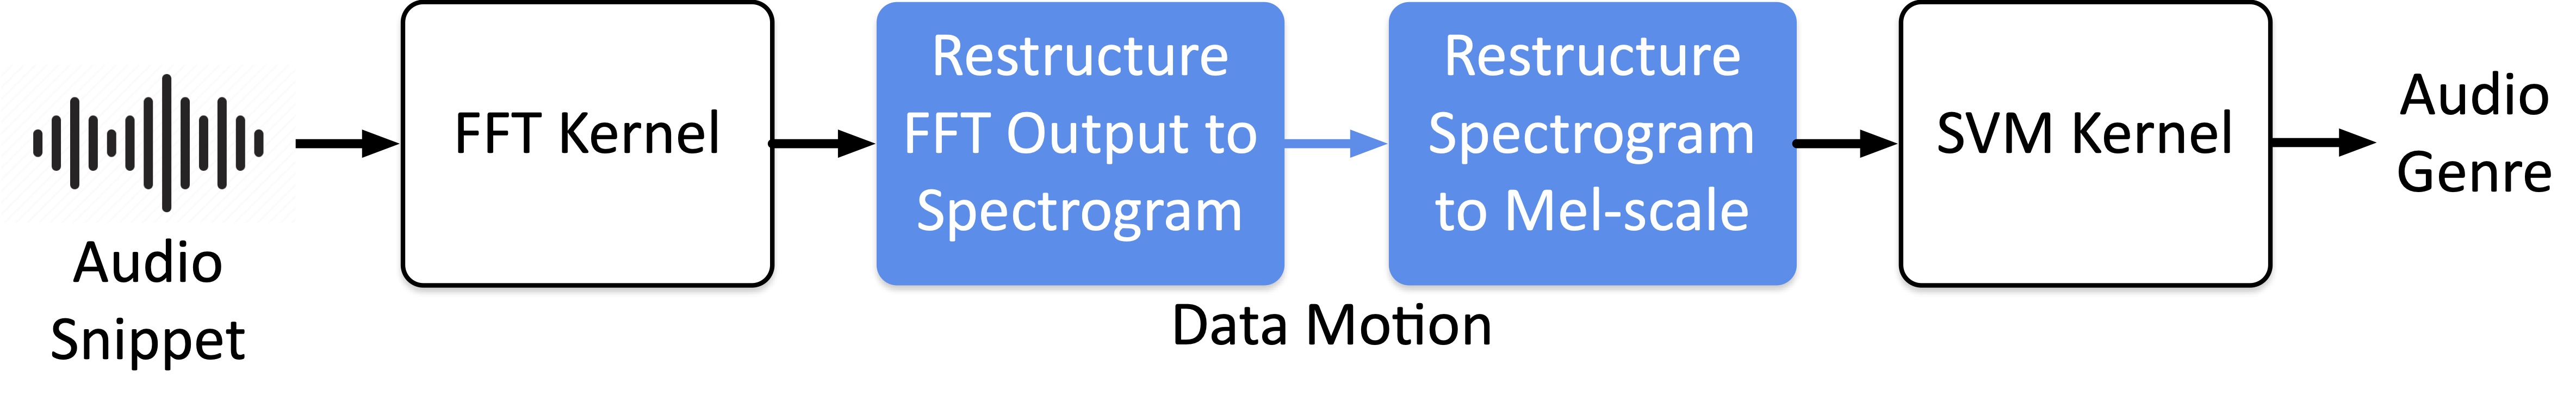
\includegraphics[width=\columnwidth]{figure/fianchetto/motivation_example_a_camera_ready.pdf}
    %\caption{Runtime breakdown when running applications on CPU or multiple accelerator setup that uses CPU for data motion.}
    \caption{}
    \label{fig:motivation:example-a}
    \end{subfigure}
    %
    \begin{subfigure}[b]{\columnwidth}
    \centering{
    \vspace{2ex}
    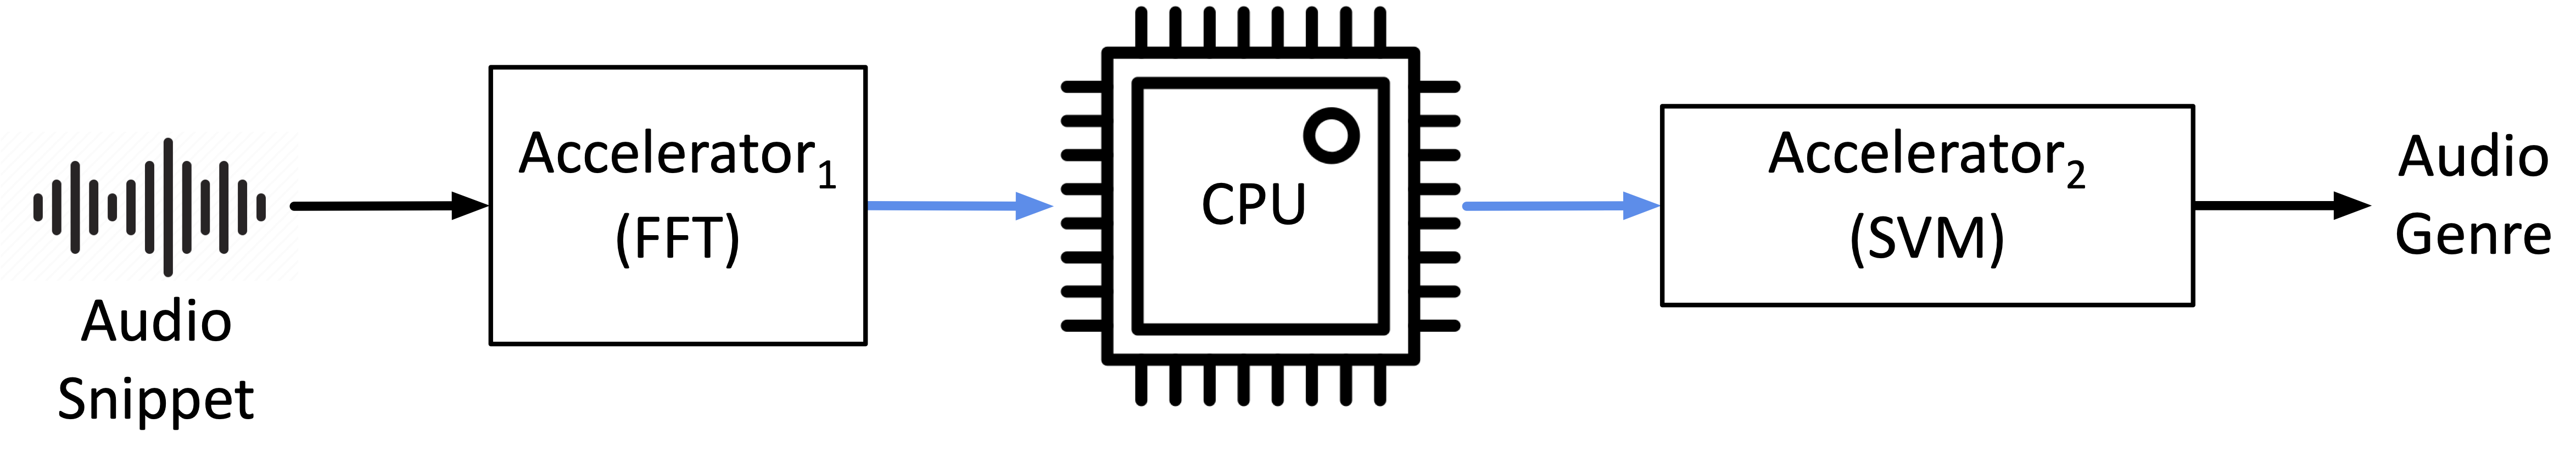
\includegraphics[width=\columnwidth]{figure/fianchetto/motivation_example_b_camera_ready.pdf}
    %\caption{Multi-acceleration performance improvement and scalability are constrained by data motion overhead.}
    \caption{}
    \label{fig:motivation:example-b}
    }
    \end{subfigure}
    %
    \begin{subfigure}[b]{\columnwidth}
    \centering{
    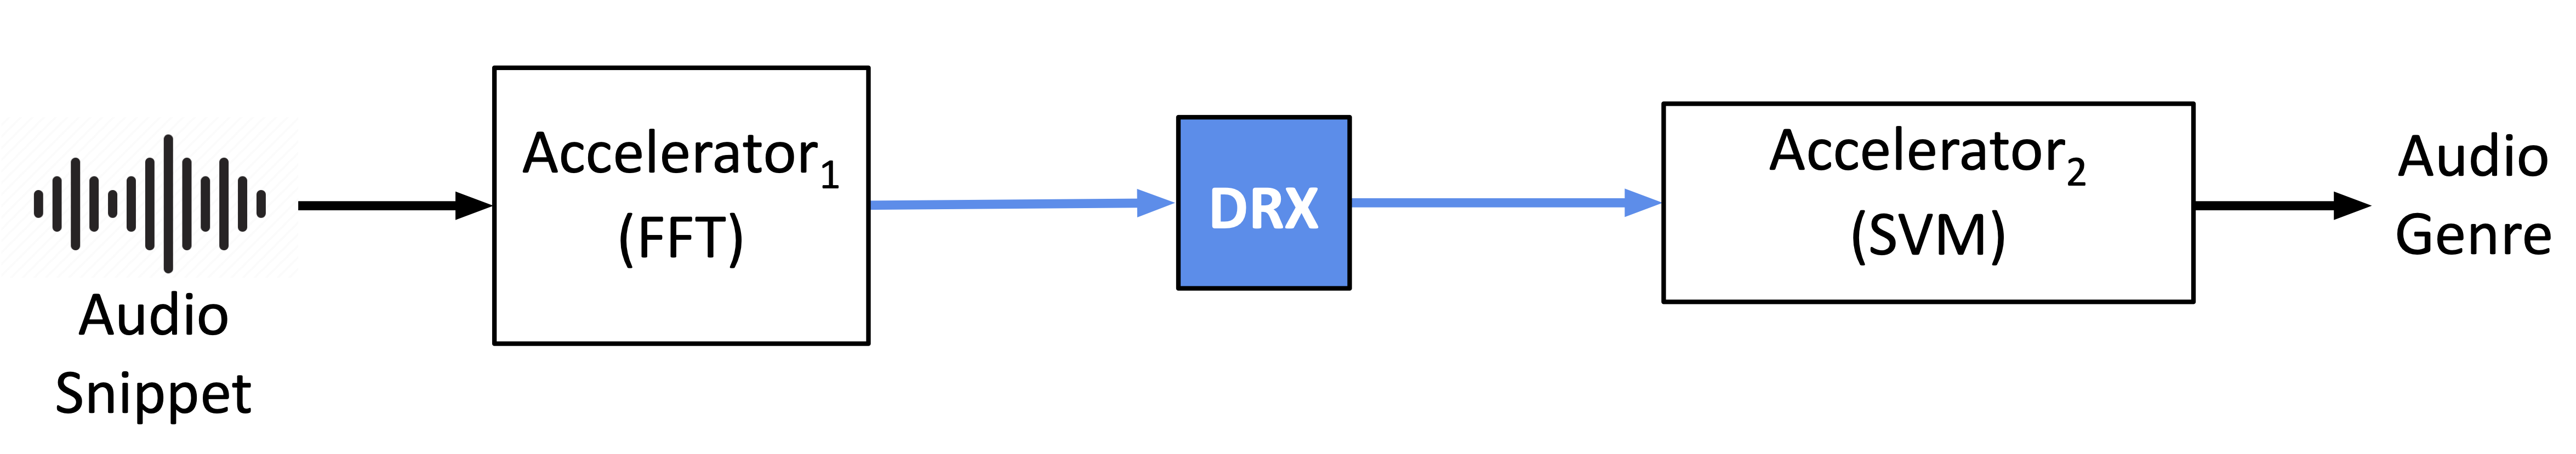
\includegraphics[width=\columnwidth]{figure/fianchetto/motivation_example_c_camera_ready.pdf}
    %\caption{Multi-acceleration performance improvement and scalability are constrained by data motion overhead.}
    \caption{}
    \label{fig:motivation:example-c}
    }
    \end{subfigure}
    % \includegraphics[width=\columnwidth]{ASPLOS23/figures-resubmit/motivation_example_camera_ready.pdf }
    \caption{ 
    (a) Data motion stands between two application kernels, i.e., Fast Fourier Transform and Support Vector Machine, of an end-to-end application.  
    %
    (b) Data motion is on CPU and application kernels are on their corresponding accelerators 
    %
    (c) For \dmx, data motion is accelerated on \drx and application kernels are on their corresponding accelerators.
    }
    \label{fig:motiv-ex}
    \vspace{-3ex}
\end{figure}

\subsection{Data Restructuring Operations}
\label{sec:motivation:operations}


In this work we use five end-to-end applications that span multiple domains~\cite{acc-yolov3:iscas:2020, urbansound-dataset:mm:2014, rldbs:ijcai:2020, microsoft-presidio,doppiodb:fpl:2017,chiosa:pvldb:2022} to quantify the inefficiencies of cross-domain acceleration in current multi-accelerator systems. Each of them has different domain-specific kernels and data restructuring requirements between the kernels. 
%
Specifically, \bench{Video Surveillance} decodes input video streams into video frames and passes them to an object detection kernel~\cite{yolov3}.
%    
\bench{Brain Stimulation} receives electromagnetic signal input generated from a brain simulation model, processes it with FFT and data restructuring operations before outputs the data to reinforcement learning kernel~\cite{rldbs:ijcai:2020}.
%   
\bench{Personal Information Redaction} decrypts privacy-sensitive text and uses a regular expression kernel to detect personally identifiable information and redact them from the text with blanks~\cite{microsoft-presidio}.
%    
\bench{Database Hash Join} decompresses database tables and hash joins the tables~\cite{doppiodb:fpl:2017,chiosa:pvldb:2022}.   

Figure~\ref{fig:motiv-ex}(a) illustrates the end-to-end application pipeline of the \bench{Sound Detection} application. %, which receives an audio snippet and detects its genre. 
%
As shown, \bench{Sound Detection} is composed of two domain-specific kernels:
%
(1) FFT kernel running short-time Fourier transformation for the input audio snippet, and
%
(2) support vector machine kernel to decide the genre of the audio snippet.
%
An intermediate \textit{data motion} step is required for restructuring the output of the FFT kernel to the input format of the support vector machine kernel while copying the data from the output buffer to the input buffer. 
%
In this example, data restructuring requires generating a spectrogram from the output of FFT kernels and applying mel scale transformation to the spectrogram. 
%
The mel scale transformation maps the spectrogram into mel-frequency bins which are closer to the human-perceivable scale.
%

%\malian{@Shu-Ting - add a few sentences explaining Table.\ref{table:data-trans-ops}}\stingw{Done}
%
%Table~\ref{table:data-trans-ops} presents five end-to-end applications~\cite{acc-yolov3:iscas:2020, urbansound-dataset:mm:2014, rldbs:ijcai:2020, microsoft-presidio,doppiodb:fpl:2017,chiosa:pvldb:2022} including \bench{Sound Detection}. Each of them has different kernels and data restructuring operations between the kernels.


%\begin{figure}[h]
\begin{subfigure}[b]{\columnwidth}
\includegraphics[width=\columnwidth]{ASPLOS23/figures-resubmit/motivation-scaling-breakdown.pdf}
%\caption{Runtime breakdown when running applications on CPU or multiple accelerator setup that uses CPU for data motion.}
\caption{}
\label{fig:motivation:bar:breakdown}
\end{subfigure}
%

\begin{subfigure}[b]{\columnwidth}
\centering{
\includegraphics[width=0.65\columnwidth]{ASPLOS23/figures-resubmit/motivation-multiaxl-constraint.pdf}
%\caption{Multi-acceleration performance improvement and scalability are constrained by data motion overhead.}
\caption{}
\vspace{-2pt}
\label{fig:motivation:bar:multiaxl}
}
\end{subfigure}
\caption{(a) Runtime breakdown when running applications on CPU or multiple accelerator setup that uses CPU for data motion. (b) Multi-acceleration speedup and scalability are constrained by data motion overhead.}
\label{fig:motivation:bar}
\end{figure}
\begin{figure}[ht!]
    \begin{subfigure}[b]{0.9\columnwidth}
    \includegraphics[width=\columnwidth]{figure/fianchetto/motivation-multiaxl-breakdown.pdf}
    %\caption{Runtime breakdown when running applications on CPU or multiple accelerator setup that uses CPU for data motion.}
    \caption{}
    \label{fig:motivation:bar:breakdown}
    \end{subfigure}
    %
    
    \begin{subfigure}[b]{0.9\columnwidth}
    \centering{
    \includegraphics[width=0.65\columnwidth]{figure/fianchetto/motivation-multiaxl-constraint.pdf}
    %\caption{Multi-acceleration performance improvement and scalability are constrained by data motion overhead.}
    \caption{}
    \vspace{-2pt}
    \label{fig:motivation:bar:multiaxl}
    }
    \end{subfigure}
    \caption{(a) Runtime breakdown when running applications on CPU or multiple accelerator setup that uses CPU for data motion. (b) Multi-acceleration speedup and scalability are constrained by data motion overhead.}
    \label{fig:motivation:bar}
\end{figure}


\subsection{Data Motion Overheads}
%
%\TODO{explain we use geomean valus acorss 5 apps but not individual apps}
Figure~\ref{fig:motivation:bar}(a) shows the geometric mean of the runtime breakdown for the five %Sound Detection application as well as four other 
applications explained in Sec.\ref{sec:motivation:operations}. We show the results for co-running up to 15 applications on the server while data restructuring is performed on the CPU. \emph{All-CPU} configuration runs application kernels on the CPU while \emph{Multi-Axl} runs the application kernels on the DSAs. Because each application consists of 2 domain-specific kernels, 15 application setup runs on 30 DSAs.
%under two scenarios: the application runs entirely on the CPU (All-CPU setup shown in Fig.\ref{fig:motivation:bar:cpu}) and the application kernels run on accelerators with PCIe interface but Data Motion runs on the CPU (Multi-Accelerator setup shown in Fig.\ref{fig:motivation:bar:accel}). Fig.\ref{fig:motiv-ex}-(b) illustrates the Multi-Accelerator setup. The numbers on the X-axis show the number of concurrent applications running on the systems. We isolate the cores that run application kernels in the All-CPU setup and dedicate 16 cores to Data Motion for both All-CPU and Multi-Accelerator setups. 
%\malian{@Shu-Ting explain the setup in detail. What part of the application is accelerate etc. What is 1 kernel , 5 kernel ... shown in the figures}
%
As Figure~\ref{fig:motivation:bar}(a) shows, in the \emph{All-CPU} setup, the execution of domain-specific kernels accounts for up to 78.5\% and on average 49.1\% of the total runtime.
%
However, the \emph{Multi-Axl} setup reduces the runtime of domain-specific kernels, but at the same time amplifies the ratio of data motion within the end-to-end runtime.
%\malian{ppl will ask what about a middle ground of using a GPU and map both kernels to run on a single GPU (review-E)?}
%
The ratios range from 71.3\% to 97.1\%, showing that data motion becomes the performance bottleneck under multi-acceleration.
%
%The efficiency of data motion determines the end-to-end performance of multi-accelerated applications. This motivates the necessity of data motion acceleration. 
%Therefore, data motion acceleration becomes a timely challenge to unleash the full benefits of multi-acceleration.
%

Another important observation from Figure~\ref{fig:motivation:bar} is the poor scalability of current multi-accelerator systems when concurrently running applications on multiple accelerators. 
%1. 1-> 5, data movement bottleneck on the CPU -> accelerator link.
From a single application to 5 applications, data movement emerges as a bottleneck. The limited PCIe bandwidth of CPUs creates a bottleneck for data moving in and out of CPU for data restructuring operations as they cannot directly connect all accelerators concurrently. %\krishnan{to themselves or concurrently?}.
%2. 5->10 and 15, data restructuring on CPU accounts for more portion of end-to-end runtime.
As the number of applications grows further to 10 and 15 applications, the CPU demonstrates its incapability to keep up with the increased concurrency of data restructuring operations though using 16 Xeon cores. % out of 20 physical cores on a Xeon server processor.
%
Such a bottleneck in data movement and data restructuring stifles the end-to-end speedup achieved by multi-acceleration at scale. As shown in Figure~\ref{fig:motivation:bar}(b), accelerating application kernel while relying on the CPU for data restructuring achieves 1.4$\times$ and 1.1$\times$ end-to-end speed up for 1 and 10 applications, while the geometric mean of per DSA speedup is 6.5$\times$. %\TODO{write about limited speedup shown in Figure~\ref{fig:motivation:limited-speedup}}
%
% The speedup of multi-acceleration with ideal data motion acceleration can be projected by Amdahl's law.
% %
% As shown in Figure~\ref{fig:motivation:ideal-speedup}, an ideal data motion acceleration offers 5.1x speedup for multi-acceleration and an overall 23.9x speedup compared to All-CPU baseline.
%

The above results demonstrate the untapped potential of multi-acceleration with ideally accelerated data motion.
%
This significant performance difference between end-to-end and per-kernel speed-up stems from the following \textbf{I}nsights:
%
\textbf{(I1)} Using specialized accelerators reduces the runtime of kernels significantly, shifting Amdahl's bottleneck towards data motion.
%
\textbf{(I2)} Host CPU engagement imposes inevitable data communication with accelerators, adding the cost of data movement on top of data restructuring.
%
\textbf{(I3)} Heterogeneity in the architecture of both accelerators and CPU demands additional data type conversions and layout transformation on top of discussed data restructuring, further amplifying the cost of data motion.
%
Heeding these insights, this work makes a case for accelerating the data motion.
%
%This paper sets out to seize this rather overlooked opportunity and introduce the new concept of data motion acceleration through careful design of system layer and hardware specialization without changing the way the current multi-accelerator systems are being programmed.
%

\section{\dmx: Accelerating the Data Motion}
\label{sec:dmx}
% \begin{comment}
% \stingw{dump notes here:
% 1. control plane is still on CPU with polling → we don’t include the software overhead of the data movement
% 2. Assume a userspace/kernel bypassing poll mode driver
% 3. we should include (1) the overhead of first loading data onto the accelerator (DMA time)
% (2) last load data back to main memory (DMA time), (3) control overhead of polling (See Pond paper for exact latency number)
% }
% \end{comment}

Multi-acceleration in Figure~\ref{fig:motiv-ex}(b) represents the current system design using CPU for data motion. This design requires data to move through the CPU for restructuring the output of one accelerator before the data can be used by the next accelerator. 
%
In this chapter, we propose Data Motion Acceleration as illustrated in Figure~\ref{fig:motiv-ex}(c) to facilitate data motion between heterogeneous accelerators. %\dmx avoids the unnecessary data movement between CPU and accelerator and accelerates the non-trivial operations of data restructuring.
%
\dmx accelerates data restructuring and bypasses CPU for data movement between accelerators via integrating the purposefully-built Data Restructuring Accelerator (\drx) into the system.
%
%achieves this goal by accelerating the execution of data restructuring, and offloading the data movement from CPU when multiple accelerators communicate with \hanyang{add software} and a purpose-built Data Restructuring Accelerator (DRX).}
%
%Accelerating the data restructuring motivates the design of a Data Restructuring Accelerator (DRX), purpose-built for executing data restructuring operations. 
%Fig.~\ref{fig:motiv-ex}-(c) illustrates a two accelerator setup with \dmx.  %The location and integration of the data motion accelerator with other accelerators directly impact the overall data movement.
%
Realizing \dmx requires synergistic design considerations at the following levels: % of (1) \drx placement, (2) system integration and programmability, (3) specialized hardware design:
%
%\stingw{structure is okay, namding of drx and dmx might change later, use macro}
\begin{itemize}
\item \textbf{\drx Placement. }
%\stingw{make sure this is consistent with the updated DRX placement in Sec.~\ref{sec:design}}
%
An important design decision in \dmx is the location of the \drx. 
%
The placement of DRX impacts the data movement and the overall system design.
%
We consider three different placements for \drx: integration on the CPU, standalone PCIe-attached card, and per accelerator bump-in-the-wire placement. 
%
% The placement of \drx impacts the data movement and the overall system stack design.

\item \textbf{Specialized Hardware Acceleration.}
%
We need to design \drx to be programmable and support a range of data restructuring operations. 
%%As Figure~\ref{fig:motivation:bar:accel} 
As Figure~\ref{fig:motivation:bar}(a) shows, data restructuring accounts for 57.7\%$\sim$73.2\% of end-to-end runtime, therefore efficient execution of data restructuring is critical for multi-acceleration.  

\item \textbf{System Integration and Programmability.}
%
%\TODO{first explain how current multi-acceleration works, and then we take it from there, with minimal changes to the way we program it. it needs to be usable otherwise it's useless}
%\stingw{make sure this is consistent with the updated system design especially the programming model}
%
To minimize data movement, the CPU should be removed from the data path of accelerator-to-accelerator communication. 
%
However, the control plane should run on the CPU, otherwise, it requires a completely new programming interface that stifles interoperability of \dmx across arbitrary accelerators.
%
In Sec.\ref{sec:system} we explain the current programming interface of multi-accelerator systems and how \dmx only offloads the data plane to the hardware without changing the current control plane.  

\end{itemize}


In Sec.\ref{sec:placement} we explore various placements for \drx and show that tight integration of \drx and accelerators in a bump-in-the-wire fashion minimizes the data movement and delivers the best performance and energy efficiency at scale. 
%
%
Next, we demystify the data restructuring operations in Sec.\ref{sec:accelerator} and introduce a programmable accelerator specialized for the data restructuring domain. 
%
Lastly in Sec.\ref{sec:system}, we discuss the runtime and kernel drivers that coordinate the offload of data restructuring operations to bump-in-the-wire \drx while still running the control plane on the CPU. 

\section{\drx Placement}
\label{sec:placement}

The key design considerations in designing \dmx are the placement of \drx and interconnection between \drx, accelerator, and CPU in the system.
%
Since \dmx is to enable interoperability between accelerators designed by different vendors, \drx's interconnect should be standard and well adopted.
%The interconnect needs to have been well-adopted for most of the devices and accelerator cards.
%
As such, the current incarnation of \dmx considers PCIe as the standard interconnect to connect accelerators to CPU and \drx. 
%
PCIe is a well-established standard of interconnect and serves as the basis for future interconnects such as CXL~\cite{cxl-3-0-spec}.  
% battleground-tested technology and future interconnects such as CXL are built atop PCIe physical layer~\cite{cxl-3-0-spec}. \hanyang{Not clear, you should say something like PCIe is industry-standard (possible one citation) and future prove (the CXL example you provided)}
%

The placement of \drx ideally should (1) scale with the capacity of associated accelerators, (2) avoid being the bandwidth bottleneck when accelerators transfer/receive data from it, and (3) minimize data movement as data movement is the main performance and energy bottleneck in today and future system~\cite{horowitz:isscc:2014}.

\begin{figure}[ht!]
    \centering
    \includegraphics[width=0.90\columnwidth]{figure/fianchetto/drx_cpu_config_camera_ready.pdf}
    \caption{Integrated \drx.}
    \label{fig:integrated-drx}
\end{figure}

%\noindent \textbf{\drx integrated with CPU.}
\noindent \textbf{Integrated \drx into CPU.}
This configuration considers integrating \drx with the CPU as illustrated in Figure~\ref{fig:integrated-drx}. 
%Figure~\ref{fig:integrated-drx}. 
%
The integrated accelerators become more common recently as Intel Sapphire Rapids, IBM z15, POWER9, and Telum offer them in their CPU products~\cite{intel-sapphire-rapids:hotchips:2021,ibm-compression-accelerator:isca:2020,ibm-telum-processor:isca:2022}.
%
Integrated accelerators are efficient in performing computation on the data that is on the CPU chip. However, integrated accelerators are going to eat up the already limited CPU power budget~\cite{dark_silicon_isca2011,dark_silicon:babak}. 
%suffer from the limited power budget as CPUs are often operating at tight power and thermal constraints~\cite{dark_silicon_isca2011,dark_silicon:babak}. \malian{SAY: accelerators are going to eat up the CPU power budget.}
%These accelerators are convenient to use as they are integrated into the CPU but this also limits the amount of power it can consume. The accelerator when running on IBM POWER 9 draws 33 Watts active power. 
%
Such power and thermal constraints limit the performance of integrated accelerators on the CPU.
%
% For example, 
% % the compression unit in IBM POWER 9 is limited to 33 Watts of active power~\cite{ibm-compression-accelerator:isca:2020} and 
% Intel Sapphire Rapids can only activate up to a fixed amount of accelerators~\cite{supermicro-sapphire-rapids}. \stingw{for supermicro servers, they can activate up to 12 from 4 types of accelerators, QAT, DLB, DSA, and IAA.} \krishnan{see comments in my email}
%

\dmx considers a fixed power budget 
%\krishnan{can't we just say -- We consider a fixed power budget -- instead of specifing it to be 34 Watts?} 
for an integrated accelerator and design an Integrated \drx to operate within this power limit~\cite{supermicro-sapphire-rapids, ibm-compression-accelerator:isca:2020}.  
%
% 34 Watts derived from the active power when IBM compression accelerator running max workload on POWER9 CPU~\cite{ibm-compression-accelerator:isca:2020}.
%\stingw{34 Watts derived from the active power when IBM compression accelerator running max workload on POWER9 CPU. }
%
%For integrated \drx, only a fixed amount of \drx hardware based on the exact power of \drx can be placed on the CPU.   
%
This fixed power budget limits the performance of \drx.
%
As we will show in Sec.\ref{sec:results}, Integrated \drx becomes the performance bottleneck when scaling the number of accelerators to more than 8.
%    
Although integrating \drx %as a separated die 
using die-to-die interconnects like UCIe could alleviate the affect, integrated \drx still becomes the performance bottleneck with excessive data movement~\cite{amd-chiplet:isca:2021, odsa-bow-spec, ucie-spec}.
%This fixed amount prevents \systemName to further scale the compute from \drx to match up with the data restructuring demand from accelerators.
%
Moreover, Integrated \drx has the same data movement as the baseline CPU without \drx. Such design requires all accelerators to send their data to the CPU which makes the PCIe link connecting the CPU to the accelerators the bandwidth bottleneck when multiple accelerators use \drx at the same time. Such data movement is also the main source of system energy consumption. %PCIe switches creates bandwidth oversubscription that force accelerators to share their bandwidth to move data in and out of \drx on the CPU.
%Moreover, \drx integrated with CPU imposes a bandwidth bottleneck when PCIe switches are introduced to accommodate the growing number of accelerators. PCIe switches creates bandwidth oversubscription that force accelerators to share their bandwidth to move data in and out of \drx on the CPU.

\begin{figure}[ht!]
    \centering
    \includegraphics[width=0.90\columnwidth]{figure/fianchetto/drx_pcie_config_camera_ready.pdf}
    \caption{Standalone \drx. Number of \drx units in Standalone placement is configurable, and the illustration represents just one possible configuration.}
    \label{fig:standalone-drx}
\end{figure}

\noindent\textbf{Standalone \drx as a PCIe card.}
This configuration considers implementing \drx as a standalone PCIe card that is installed just like any other accelerator on a PCIe slot. 
%aggregating a certain units of \drx hardware.  
%
%The advantage of the standalone \drx is the higher power budget of a PCIe card compared with an integrated \drx. 
%
Without using an external power supply cable, the performance of a single Standalone \drx PCIe card is limited by the PCIe power supply standard, which is 25 Watts, and its bus bandwidth.
%
Nevertheless, as illustrated in Figure~\ref{fig:standalone-drx}, installing multiple Standalone \drx cards can scale \drx performance with the number of accelerators. 
%resolves the power limit imposed by CPU integration and further the scale of \drx to match up with the number of accelerators.  
%
However, this Standalone \drx still incurs bandwidth oversubscription as the PCIe link to a shared, Standalone \drx card can become the bottleneck.
%
The bandwidth contention could be worse with multiple Standalone \drx cards are under the same PCIe switch. 
%However, this Standalone \drx still incurs bandwidth oversubscription as accelerator accessing a piece of shared hardware below a PCIe switch.
%

Compared to Integrated \drx, a Standalone \drx has the potential to reduce the data movement if \dmx implements a point-to-point PCIe connection between \drx card and accelerator cards. This way, a Standalone \drx can localize the communication under the PCIe switch to which other accelerator cards are installed. 
%\hanyang{So is it implemented this way in the experimental setup? If not the speedup/energy reduction should not be scaling with the application count in the standalone configuration, if so, you shouldn't say it has the potential, just say it does}
%\stingw{something more exactly about how its bandwidth oversubscription is different from CPU's case.}
%\stingw{we still have BITW but we'll have a internal PCIe switch like Samsung SmartSSD shown in their documentation.~\cite{samsung-smartSSD:documentation:2020}}

\begin{figure}[ht!]
    \centering
    \includegraphics[width=0.90\columnwidth]{figure/fianchetto/drx_pcie_switch_config_camera_ready.pdf}
    \caption{PCIe-Integrated \drx.} 
    \label{fig:drx-config-on-pcie-switch}
\end{figure}

\noindent\textbf{PCIe-Integrated \drx.}
This configuration integrates \drx onto a PCIe switch (Shown in Figure~\ref{fig:drx-config-on-pcie-switch}).
%
%Compared to a Standalone \drx, A PCIe-Integrated \drx saves a round-trip between the source \drx and the source PCIe switch and a pass through the destination PCIe switch.  
Compared to a Standalone \drx, A PCIe-Integrated \drx saves a round-trip between \drx and the PCIe switch.  
%
However, PCIe-Integrated \drx requires \drx to operate at the aggregated rate of all downstream PCIe ports, which adds considerable hardware complexity. 
%
Also, computation on switches only permits limited memory usage and a limited number of instructions per packet~\cite{rmt:sigcomm:2013,drmt:sigcomm:2017,in-network-compute:hotnets:2017,in-network-compute:eurosys:2019}. 
%
This configuration requires significant engineering effort to redesign the PCIe hardware and related software stack. 

\begin{figure}[ht!]
    \centering
    \includegraphics[width=0.90\columnwidth]{figure/fianchetto/drx_acc_config_camera_ready.pdf}
    \caption{Bump-in-the-Wire \drx.
    }
    \label{fig:drx-config-acc}
\end{figure}

\noindent\textbf{Bump-in-the-Wire \drx.}
Lastly, we introduce a Bump-in-the-Wire \drx configuration 
inspired by Catapult~\cite{catapult:isca:2014} that connects an exclusive \drx to each accelerator (Figure~\ref{fig:drx-config-acc}).

Bump-in-the-Wire configuration avoids overprovisioning of PCIe links and \drx resources for a multi-accelerator system and enables \dmx to scale with the hardware resources compared with the other configurations.
%
More importantly, Bump-in-the-Wire \drx placement reduces the data movement to a minimum when accelerators communicate with each other.
%
%Accelerators and their \drx can be tightly integrated on the same chip with unified memory to avoid any data movement between them. 
%
Coupled with a programmable \drx that enables offloading of any data restructuring operation (c.f., Sec.\ref{sec:accelerator}), Bump-in-the-Wire \drx serves as an option to build future scalable multi-accelerator systems.


\section{Data Restructuring Accelerator (\drx) Design}
\label{sec:accelerator}

As discussed in Sec.\ref{sec:motivation}, the CPU is not an optimal place to perform data restructuring operations. 
In this section, we first analyze different data restructuring operations by profiling their execution on the CPU. This analysis guides us in devising a programmable accelerator specialized for the data restructuring domain. Refer to Sec.\ref{sec:method} for more information on the experimental setup. %Then we use the insights to devise a programmable accelerator specialized for the data restructuring domain. 

\begin{figure}[ht!]
    \centering    
    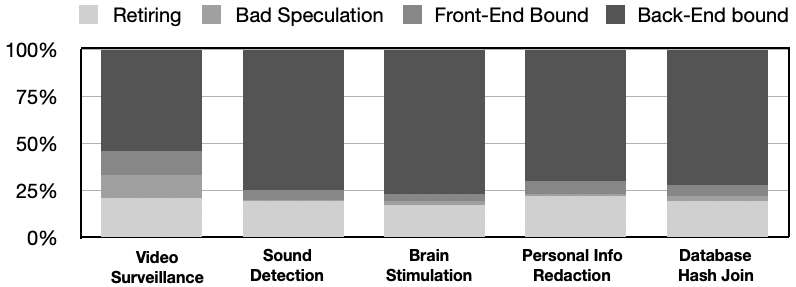
\includegraphics[width=0.9\columnwidth]{figure/fianchetto/profiling_vtune.pdf}
    \caption{Top-down breakdown of stall cycles for data restructuring operations.}
    \label{fig:topdown}
\end{figure}

\subsection{Data Restructuring Characterization}
%We profiled the five representative data restructuring operations explained in Sec.\ref{sec:motivation:operations}. 
%
%The data restructuring operations are implemented using PyTorch which uses Intel oneAPI Math Kernel Library (MKL). MKL transparently vectorizes data restructuring operations when running on a CPU by using AVX-256, AVX-512, or newer SIMD instructions. 
%
%We use Intel Vtune Profiler~\cite{vtune} to profile the operations and list several observations. These observations guide our design of \drx. Refer to Sec.\ref{sec:method} for more information on the experimental setup. 
Figure~\ref{fig:topdown} shows the top-down~\cite{top-down:ispass:2014} breakdown of stall cycles for data restructuring operations. 
%\malian{cite top down paper: https://ieeexplore.ieee.org/document/6844459} 
%
We characterize data restructuring operations with the top-down analysis of Intel VTune~\cite{intel-vtune} on an Intel Xeon Gold 6242R processor. 
%
The processor has the same microarchitecture as our testbed setup on AWS (See Sec.\ref{sec:method} for details).
%
%As shown, the operations are either waiting for the backend or retiring. 
Across different data restructuring operations, we see at most 12.5\% Bad Speculation Bound and 14\% Front-End Bound cycles. A deeper analysis of \textit{Video Surveillance} reveals that this distinct behavior is linked to a higher number of branch instructions, resulting in a relatively larger number of cycles spent on branch re-steer and uOp cache switches. On the other hand, the Back-End Bound cycles range from 53\% to up to 77.6\% of total cycles. The culprit for Back-End Bound cycles is both the unavailability of functional units and misses in the data cache. 23.2\% of Back-End Bound cycles are Core-Bound and 46\% are Memory-Bound. %Because the data restructuring operations have plenty of data level parallelism, the Top-Down breakdown suggests that they are contending for functional units and waiting for memory. 

The profiling shows that data restructuring operations have low L1I cache Misses Per Kilo Instructions (MPKI). The average L1I MPKI for data restructuring is 2.3. As a reference, our measurements for online services from CloudSuite~\cite{noauthor_cloudsuite_nodate} report an average of 7.8 L1I MPKI. 
%0.1$\sim$4.1 
%with an average while MPKI of SPEC 2017\cite{speccpu2017} is 0.1$\sim$11.6~\cite{panda_wait_2018}. 
Such low L1I MPKI suggests a small instruction working set for data restructuring operations that fit inside the L1I cache of the core. 

%\noindent{\textit{Observation3: data restructuring operations have plenty of data-level parallelism.}}

The profiling results show that all data restructuring operations have a high degree of vector unit utilization. The data restructuring kernels use 100\% of available vector unit capacity which is 256 bits wide AVX-256 on our servers. 
%However, we observe that the data restructuring kernels can only utilize 50\% of the available vector unit capacity. This is because the %vector operations are 256 bits wide while the Xeon CPU implements 512-bit wide vectors. 
We also observe a high number of ephemeral threads that are spawned by the Intel Math Kernel Library while restructuring the data. The number of threads that are spawned while running the data restructuring operations is between 130 to 140. These threads operate on the data in parallel and illustrate the high data-level parallelism and inefficiency of CPUs in executing the data restructuring operations.

%\vspace{-2ex}
\subsection{\drx Hardware Architecture}
We use the above insights to design a programmable \drx that specializes in the data restructuring domain.
%
The main observations driving \drx design are the abundance of data-level parallelism, streaming access pattern, and non-trivial operations of data restructuring. Figure~\ref{fig:drx-acc-arch} overviews the architecture of \drx hardware.
%

\drx uses a decoupled access-execute architecture that consists of a programmable front-end specialized for walking over multi-dimensional data structures, and a configurable number of interleaved vector processing units dubbed Restructuring Engine (RE) in the same pipeline. 
%
It also includes a Transposition Engine for data transposition operations and a programmable Off-chip Data Access Engine for off-chip load/store which also houses a DMA engine that initiates data movement with other accelerators.  %128-lane 256-bit vector processing unit dubbed Restructuring Engine (RE) in the same pipeline. It also includes a Data Transposition Engine to ensure full coverage of data transposition scenarios. 
%
For evaluation, we configure the \drx to contain 128 lanes of RE, a 64KB instruction cache, a 64KB data scratchpad, and 8GB of DDR4 DRAM.  %\malian{should we make it 8GB considering that we need more memory to map buffer for DRX-DRX communication?}. 
A DDR4 3200 memory channel sustains $\sim$25GBps, therefore \drx implements a single DDR4 channel to match the bandwidth of an x8 PCIe Gen 4 link.%\malian{for the evaluation we use these. Seperate the general design and then one for specification.}
%
% When issuing instructions to \drx REs, the Instruction Repeater in the front-end tracks the loop iteration and calculates the scratchpad addresses based on the configuration stored in Strided Scratchpad Address Calculation, eliminating the need for vector register files and issuing excessive numbers of memory instructions.
% %
% Instead, the data is fetched from the interleaved scratchpads in the REs based on pre-computed addresses by the front-end. 
% %
% A programmable Off-chip Data Access Engine connects these scratchpads for DRAM load/store, the Off-chip Data Access Engine also houses the DMA engine that initiates data movement with other accelerators. 
% %

\noindent \textbf{\drx ISA. }
The DRX ISA and hardware architecture are optimized based on the observation that data restructuring workloads consist of known-shape, pre-located multidimensional arrays. Such arrays can be indexed using a set of loops. As shown in Figure~\ref{fig:drx-acc-isa}, the DRX ISA includes specialized loop, compute, off-chip memory access, and synchronization instructions for vector operations while preserving the option for scalar operations, enabling serial tasks like pointer dereferencing.

%DRX ISA and hardware architecture are optimized based on the observation that data restructuring workloads consist of known-shape, pre-located multidimensional arrays, and such multidimensional arrays can be indexed with a set of loops.
%
%As such, DRX ISA consists of loop, compute, off-chip memory, and synchronization instructions that are specialized for vector operation while still preserving the option to operate on scalar, which enables serial operations such as pointer de-reference.
%
The DRX ISA significantly departs from traditional SIMD semantics, offering optimizations for memory, loops, and data packing. 
%
For memory optimization, DRX employs software-managed on-chip scratchpads instead of vector register files and the conventional cache hierarchy found in common SIMD ISAs. 
%
Memory instructions configure the Off-chip Data Access Engine to fetch data directly from DRAM to the on-chip scratchpads. 
%
For loop optimization, DRX utilizes hardware loops within an Instruction Repeater unit to reduce branch instruction overhead. 
%
Loop instructions configure the Instruction Repeater based on the dimensions of the kernel's multidimensional arrays. 
%
For data packing optimization, the DRX compiler partitions the kernel's multidimensional arrays across the REs, eliminating the need for pack/unpack instructions.

%DRX ISA is a significant departure from the traditional SIMD semantics and offers optimization for memory, loop, and data packing. For memory optimization, DRX uses software-managed on-chip scratchpads instead of vector register files and conventional cache hierarchy in common SIMD ISA. Memory instruction configures the Data Access Engine to fetch data from DRAM directly to on-chip scratchpads. For loop optimization, DRX uses hardware loops within Loop Repeater to eliminate branch instruction overhead. Loop instructions configure the Instruction Repeater based on the dimensions of kernel multidimensional arrays. For data packing optimization, the DRX compiler partitions the kernel multidimensional arrays across the REs to eliminate the need for pack/unpack instructions. 

During the vector execution, loop instructions first configure the Off-chip Data Access Engine and Strided Scratchpad Address Calculator with sets of (Base, Stride, Iteration) configurations that correspond to the input/output loop dimensions and data location. 
%
After the Off-chip Data Access Engine loads the data to scratchpad banks, compute instruction is issued with scratchpad addresses calculated by the Instruction Repeater by traversing the dimensions of multidimensional arrays based on the configurations in the Strided Scratchpad Address Calculator. 
%
This data access scheme significantly reduces memory and address calculation overhead and is applied to all operations on multidimensional arrays such as data transformation, memory access, and compute operations. 
%
Finally, synchronization instructions are issued at the start and the end of the instruction stream to ensure proper program order. For scalar execution, \drx turns off all but one REs and operates as a scalar in-order CPU. 


\begin{figure}[ht!]
    \centering
    \includegraphics[width=0.9\columnwidth]{figure/fianchetto/drx-acc-arch.pdf}
    \caption{DRX Hardware Architecture.
    }
    \label{fig:drx-acc-arch}
    \vspace{-2ex}
\end{figure}

\begin{figure}[ht!] 
    \centering
    \includegraphics[width=0.9\columnwidth]{figure/fianchetto/drx-acc-isa.pdf}
    \caption{DRX instruction types.}
    \label{fig:drx-acc-isa}
\end{figure}

\noindent \textbf{\drx compiler.}
%We design a compiler that can
Inspired from prior works~\cite{tvm:osdi18, autotvm:2018} in other domains, \drx compiler compiles high-level data restructuring kernels into \drx instructions based on the DRX ISA.
%
% \drx compiler compiles high-level high-level data restructuring operations into \drx instructions based on the ISA. 
%
The \drx compiler takes two inputs: a high-level representation of the data restructuring kernel and an architecture configuration file that defines the \drx hardware configurations such as the number of REs and on-chip scratchpad size.
 %
The compiler first maps the data restructuring kernel to the intermediate representation of the kernel operations.
 %
 It then optimizes tiling and relaxes dependency on the intermediate representation based on the hardware configuration and the dimension of multidimensional arrays. 
 %
 Finally, it generates instructions based on \drx ISA from the optimized intermediate representation.
 %
 Figure~\ref{fig:drx-acc-kernel} shows a sample of the DRX kernel.
 %
 %We will open-source the compiler and DRX Verilog implementation.

 \section{System Integration and Programmability}
\label{sec:system}

In this section we discuss the system integration and programmability of \dmx with Bump-in-the-Wire DRX placement. The system integration of other DRX placements share many similarities with Bump-in-the-Wire DRX.

\noindent \textbf{Programming model.}
\dmx implements an OpenCL-style programming model that has a host program on the CPU and kernels on accelerators or \drx. 
%
Application kernels are executed on accelerators while data restructuring kernels are executed on \drx.
%
Because \dmx runs the control plane on the CPU, it does not compromise the programmer's productivity and does not incur any additional accelerator orchestration overhead compared to the baseline multi-acceleration system. % incurs the same level of system overhead as the multi-acceleration baseline because both are based on the composition of host program and kernels~\cite{opencl,xilinx-vitis-vivado:2020,oneapi}.
%}

The host program creates an execution context for each instance of the application kernel or data restructuring kernel. The context includes (1) the hardware -- e.g. the accelerator or \drx -- involved in the applications, (2) application or data restructuring kernels, and (3) a per accelerator \textit{command queue} that is mapped to the global host address space. The command queue is used for buffering the output of the application kernels and the restructured input of the next application kernel before being transferred to the destination.

The host program uses user-level OpenCL API to create the execution context. 
%
It also uses the API to interact with the accelerators and \drxs through their own \textit{command queue} on each device. 
%
The command queue accepts commands to enqueue kernels for execution, transfer data, or synchronize memory buffers. %\malian{do we talk about all these functions?} \stingw{we need the three of them here. I deleted map/unmap as we don't map memory buffer to user space in our use case.}.
%The command queues accept commands to enqueue kernel and data restructuring program for execution, transfer/synchronize memory buffers, or map/unmap memory buffer in the host memory.
%
The execution of a command can be blocking or non-blocking. 
%
Blocking execution does not return to the host program before the current command completes. 
%
Non-blocking execution, on the other hand, requires a detailed description of the dependency between kernels and data restructuring programs. 
%
For a single command queue, the queued commands are executed in the order they are enqueued.

%\dmx follows OpenCL style programming model. It considers a host connected with one or more accelerators. An application using \systemName implements host program, kernel program running on accelerators, and data restructuring program on DRX.
%
The application kernels execute domain-specific kernels of the end-to-end application on different accelerators. 
The data restructuring kernels perform the required data restructuring operations when two accelerators are communicating. The host program executes the serial portion of the application and runs a daemon to orchestrate the execution of application and data restructuring kernels running on accelerators and \drxs, respectively. 
%A host-side program orchestrates the execution of kernels and data movement, which can be between the CPU and accelerators or between accelerators. 
%
%A kernel program executes the kernel specified by the application.
%
The data restructuring kernels are shipped to \drxs that understand the exact input and output format of each accelerator. The data restructuring kernels are engaged to ensure that properly structured input/output data is moved directly between accelerators and \drx.
% \malian{You need to check how P2P works, explain it, and then define \dmx programming to follow P2P style of programming two accelerators.}

\begin{figure}[t]
    \centering
    \includegraphics[width=\columnwidth]{figure/fianchetto/drx-acc-kernel.pdf}
    \caption{Sample DRX kernel.}
    \label{fig:drx-acc-kernel}
\end{figure}

%\TODO{mention who provides the device driver-> accelerator vendor/developer}
\noindent \textbf{Driver support for \dmx.} 
At a high level, \dmx enumerates both accelerators and \drxs as PCIe devices connected to the CPU.  
%
%\dmx drivers include accelerator driver to initialize and control the accelerator cards, 
%
Each \drx unit has a driver to initialize the command queues, exchange the start and end pointers of the queue to other \drxs at the start, and orchestrate data restructuring operations. 
%
The drivers use GEM~\cite{linux-drm-gem,linux-gem-lwn} for command executions and memory-related operations. \drx driver executes commands and reads/writes/maps operations using ioctl syscall. 
%for device-specific operations.
%
For setting up point-to-point DMA between \drx and accelerators, the drivers use dma-buf API~\cite{dma_buf:kernel:2022}.
%An interconnect driver orchestrates peer-to-peer DMA between \drx and accelerator.
%
The vendor-specific accelerator drivers should support point-to-point DMA in order to work with \dmx.
%The drivers of accelerators are provided by the vendors as they contain device-specific details. 
%\stingw{NAPI-like interrupt handling is here}
By default, we operate accelerators and \drxs in interrupt mode for sending notifications to the CPU. The interrupt handling of the drivers utilizes interrupt coalescing for the bursty arrival of interrupts. 
%
If the arrival rate of interrupts exceeds a certain threshold, the drivers switch to polling. This design is similar to Linux NAPI design~\cite{napi:kernel:2022}.
% \stingw{accelerator driver:}
% It initializes the  

\begin{figure}[t!]
    \centering
    \includegraphics[width=0.9\columnwidth]{figure/fianchetto/data-queue-on-drx.pdf}
    \caption{ 
    %\drx's memory space and RX/TX data queue pairs. \drx uses the data queue as a circular buffer with head and tail pointers. \textit{$RX_{i}$} receives data from other accelerators sending its data to ${Accelerator}_{i}$. \textit{$TX_{i}$} sends restructured data from \drx to ${Accelerator}_{i}$. \drx supports up to a total $n=40$ accelerators in the current design.
    RX/TX data queue pair architecture in Bump-in-the-Wire \drx. \drx uses the data queue as a circular buffer with head and tail pointers. The output of the accelerator that is destined for ${Accelerator}_{i}$ is enqueued in \textit{$RX_{i}$} before being restructured and stored in \textit{$TX_{i}$} for transmission to ${Accelerator}_{i}$. Current \drx implementation supports up to a total $n=40$ accelerators.
    }
    \label{fig:system:data-queue}
\end{figure}

\begin{figure}[t!]
    \centering
    \includegraphics[width=\columnwidth]{figure/fianchetto/p2p_dma_workflow_camera_ready.pdf}
    \caption{Point-to-point DMA workflow involves two accelerators and the sending side \drx. 
    %
    The DMA bypasses the receiving side \drx.
    %
    \dmx supports other communication patterns such as broadcast and multicast among \drxs and between \drxs and accelerators.
    }
    \label{fig:system:p2pdma}
\end{figure}

%\noindent \textbf{\drx driver.}
Although Bump-in-the-Wire \drx is attached to each accelerator, each \drx unit should be able to set up a point-to-point connection with all the other accelerators and \drxs in the system.
%
The memory address space of each \drx is statically partitioned between all the accelerators as well as \drxs in the system to implement two pairs of RX/TX \textit{data queues} per accelerator on each \drx: one pair of queues for direct \drx-accelerator communication and another pair of queues for \drx-\drx communication.
%types of RX/TX \textit{data queues} per accelerator on each \drx: a type of queue pairs for communicating with other accelerators and another type of queue pairs for communicating with other \drxs.}
%a pair of \textit{data queues} per accelerator on each BITW \drx: RX and TX data queues.
%to serve a fixed number of accelerators. 
%

The number of accelerators is determined at PCIe enumeration time when it discovers connected accelerators that need data restructuring. We provision 8GB of memory space for implementing data queues on each \drx. The size of each data queue pair is 100MB. This will enable \dmx to support up to 40 accelerators on a server. 
%The memory address space of each \drx is statically partitioned to serve a fixed number of accelerators. 
%
\drx driver maintains a head and tail pointer for each data queue to keep track of the data that is enqueued for restructuring. 
%
RX and TX data queues on a \drx are shown in Figure~\ref{fig:system:data-queue}.
%
A point-to-point DMA moves data between data queue pairs and accelerator memory. %The memory buffer stored on \drx's memory partition is used for peer-to-peer DMA between accelerators and \drxs. 
%
% Peer-to-peer DMA enables \drx as a BITW to be passed through on the receiving side when no data restructuring operation is needed. 


GEM allocates and frees data buffers opaquely because it is agnostic to the data content in the buffer. %The driver creates memory buffers from the memory allocation of GEM. 
%
The allocated data buffers are referred to by their handle, which is equivalent to a file descriptor. %in user space for applications. 

%\noindent \textbf{Peer-to-peer DMA Among Accelerators and \drxs.}
\begin{table*}[ht!]
    \centering
    \resizebox{\textwidth}{!}{%
    \footnotesize{
    \begin{tabular}{|l|l|l|l|l|l|l|}
\hline
\textcolor{black}{Benchmark} &
  \textcolor{black}{Kernel 1} &
  \textcolor{black}{Kernel 1 Accelerator} &
  \textcolor{black}{Data Restructuring} &
  \textcolor{black}{Kernel 2} &
  \textcolor{black}{Kernel 2 Accelerator} &
  \textcolor{black}{Input Dimension} \\ 
\hline
 \begin{tabular}[c]{@{}l@{}}Video\\ Surveillance~\cite{acc-yolov3:iscas:2020}\end{tabular}&
  H.264 Codec &
  \begin{tabular}[c]{@{}l@{}}Xilinx Video\\ Codec Unit~\cite{xilinx-u30-vcu}\end{tabular} &
  \begin{tabular}[c]{@{}l@{}}Mul, MaxPool, \\ Reshape, Cast\end{tabular} &
  \begin{tabular}[c]{@{}l@{}}Object \\ Detection\end{tabular} &
  DNN Accelerator~\cite{dnnweaver:micro:2016} &
  (960, 540, 3) \\ \hline
  \begin{tabular}[c]{@{}l@{}}Sound\\ Detection~\cite{urbansound-dataset:mm:2014}\end{tabular}&
  FFT &
  \begin{tabular}[c]{@{}l@{}}Xilinx Vitis\\ DSP Library~\cite{xilinx-vitis-dsp}\end{tabular} &
  \begin{tabular}[c]{@{}l@{}}Pow, Add, Mul, \\ Div, Log10, Cast\end{tabular} &
  \begin{tabular}[c]{@{}l@{}}Support Vector \\ Machine\end{tabular} &
  \begin{tabular}[c]{@{}l@{}}Xilinx Vitis Data \\ Analytics Library~\cite{xilinx-vitis-data-analytics}\end{tabular} & 
  (8192, 768) \\ \hline
\begin{tabular}[c]{@{}l@{}}Brain\\ Stimulation~\cite{rldbs:ijcai:2020}\end{tabular}&  
  FFT &
  \begin{tabular}[c]{@{}l@{}}Xilinx Vitis\\ DSP Library~\cite{xilinx-vitis-dsp}\end{tabular} &
  \begin{tabular}[c]{@{}l@{}}Pow, Div, Mul, \\ Cast\end{tabular} &
  \begin{tabular}[c]{@{}l@{}}Proximal Policy \\ Optimization\end{tabular} &
  DNN Accelerator~\cite{dnnweaver:micro:2016}&
  (256, 1024, 8) \\ \hline
\begin{tabular}[c]{@{}l@{}}Personal Information \\ Redaction~\cite{microsoft-presidio}\end{tabular} &
  AES-GCM &
  \begin{tabular}[c]{@{}l@{}}Xilinx Vitis\\ Security Library~\cite{xilinx-vitis-security}\end{tabular} &
  Concat, Flatten &
  \begin{tabular}[c]{@{}l@{}}Regular \\ Expression\end{tabular} &
  \begin{tabular}[c]{@{}l@{}}Xilinx Vitis Data \\ Analytics Library~\cite{xilinx-vitis-data-analytics}\end{tabular} &
  (4, 2048, 768) \\ \hline
  \begin{tabular}[c]{@{}l@{}}Database Hash  Join\\ \cite{doppiodb:fpl:2017} \end{tabular} &
  Gzip&
  \begin{tabular}[c]{@{}l@{}}Xilinx Vitis Data~\cite{xilinx-vitis-data-compression} \\ Compression Library \end{tabular} &
  \begin{tabular}[c]{@{}l@{}}Concat, Reshape, \\ Cast\end{tabular} &
  Hash Join&
  \begin{tabular}[c]{@{}l@{}}Xilinx Vitis \\ Database Library~\cite{xilinx-vitis-database}\end{tabular} &
  (4, 1024, 512) \\ \hline
\end{tabular}%}}
    \caption{End-to-end benchmarks}
    %\rohan{Shu-Ting I think the data restructuring operation should be in between the kernel 1 and kernel 2}
    \label{table:benchmark}
\end{table*}

\noindent \textbf{End-to-end data motion acceleration.}
Figure~\ref{fig:system:p2pdma} shows the interactions between accelerators, CPU, and Bump-in-the-Wire \drx when $Accelerator_{1}$ tries to communicate with $Accelerator_{2}$. Although Figure~\ref{fig:system:p2pdma} depicts the accelerator and its \drx as separate chips with separate DRAM modules, \drx can be integrated into the accelerator chip and share its physical DRAM modules. %Note that  to demonstrate how \drx can be easily integrated with existing accelerators.
%
%Before any communication take place, at system boot up time, each BITW \drx communicates the data queue offset corresponding to each 
%
%The driver support of \dmx enables efficient peer-to-peer DMA workflow shown in Figure~\ref{fig:system:p2pdma}.
%
%The GEM-style system driver allocates buffers for accelerators and \drxs with backing storage on the system memory.
%
When $Accelerator_{1}$ completes kernel execution in step~\circled{1}, it raises an interrupt to the CPU in step~\circled{2}. The driver of $Accelerator_{1}$ captures the interrupt and setup a point-to-point DMA between $Accelerator_{1}$ and the TX data queue corresponding to $Accelerator_{2}$ on $DRX_{1}$.
%
$DRX_{1}$'s driver shares the offset of $RX_{2}$ data queue (i.e., RX data queue corresponding to $Accelerator_{2}$) in step~\circled{3} with $Accelerator_{1}$.
%
This enables the $Accelerator_{1}$ to access and write to the $RX_{2}$ data queue on $DRX_{1}$.
%\stingw{The execution context of \drx-0 exports, not the hardware device.}
%
A \drx driver then configures $Accelerator_{1}$ to perform a point-to-point DMA and move data from $Accelerator_{1}$'s memory to the next available buffer in $RX_{2}$ data queue on $DRX_{1}$ in step~\circled{4}.
%The host program configures the MMIO registers with source (\textit{acc-output)}) and destination buffer (\textit{acc-1-tx-data-queue}) address and then initiates peer-to-peer DMA between Accelerator-0 and \drx-0 in step~\circled{3}.
%
%In step~\circled{4}, the peer-to-peer DMA between Accelerator-0 and \drx-0 goes through the internal PCIe switch and reaches the memory address on \drx-0. 
%
The \drx processing unit on $DRX_{1}$ reads the output on $Accelerator_{1}$'s memory from $RX_{2}$ data queue, performs data restructuring, and writes the output to the next available buffer in $TX_{2}$ data queue as shown in step~\circled{5} to~\circled{7}.
%
In step~\circled{8}, $DRX_{1}$ raises an interrupt to the CPU to notify the $DRX_{1}$ driver about the completion of data restructuring.
%
Next, a point-to-point DMA is configured between $DRX_{1}$ and $Accelerator_{2}$ in step~\circled{9}.  
%is similar to step~\circled{3}.
%
In step~\circled{10}, point-to-point DMA between $DRX_{1}$ and $Accelerator_{2}$ passes through an internal PCIe multiplexer
%[MUX/switch]
without invoking $DRX_{2}$ because it does not need further data restructuring on it.
%
In step~\circled{11}, $Accelerator_{2}$ runs the kernel on its DRAM. 

\noindent \textbf{One-to-many and many-to-one data movement.} 
Supporting broadcast and multicast between the accelerator chain is necessary for load balancing as well as efficient collective communication implementation. 
%
The workflow of such movement patterns is similar to that of Figure~\ref{fig:system:p2pdma}, except that for one-to-many, the source \drx transfers the restructured output of the source accelerator to multiple accelerators (or \drxs) using multiple back-to-back point-to-point DMA transfers. 
%
Variations of many-to-one data movement can be used to implement reduction collectives by setting up direct data transfer from multiple source \drxs to a single destination \drx that also performs the reduction operation. 
%
The \dmx support for broadcast and multicast facilitates the efficient implementation of various collective operations. 


\section{Experimental Methodology}
\label{sec:method}

\noindent \textbf{Benchmarks.}
%
We create five diverse cross-domain and end-to-end applications inspired by real-world scenarios. 
%
Table~\ref{table:benchmark} lists the five benchmark applications, their cross-domain kernels and corresponding accelerators, the data restructuring operations needed to chain the kernels, and the dimensions of the input data.
%
Each application is a pipeline of two kernels, where the first kernel outputs intermediate data, which requires restructuring before it can be processed by the second kernel.
%
The \bench{Video Surveillance} decodes input video streams into video frames and passes them to an object detection kernel~\cite{yolov3}.
%
\bench{Sound Detection} performs Fast Fourier Transform (FFT) on audio snippets and use the transformed snippets to determine the genre of input audio~\cite{urbansound-dataset:mm:2014}.
%
\bench{Brain Stimulation} receives electromagnetic input signal generated from a brain simulation model, processes it with FFT and data restructuring operations before outputting the data to reinforcement learning kernel~\cite{rldbs:ijcai:2020}. 
%
\bench{Personal Information Redaction} decrypts privacy-sensitive text and uses a regular expression kernel to detect personally identifiable information and redact them from the text with blanks~\cite{microsoft-presidio}. 
%
\bench{Database Hash Join} decompresses database tables and hash joins the tables~\cite{doppiodb:fpl:2017,chiosa:pvldb:2022}.   
%
To exercise the system performance with respect to resource contention on interconnect bandwidth and compute for data restructuring, we use 1, 5, 10, to 15 concurrent running applications for the benchmarks.
%

\noindent \textbf{\drx hardware implementation.}
%
We implement \drx using Verilog in RTL and synthesize it on Xilinx UltraScale+ VU9P FPGA using Xilinx Vivado 2022.2. The synthesized design achieves an operating frequency of 250 MHz. We also synthesize an ASIC version of \drx using Synopsys Design Compiler R-2020.09-SP4 with the FreePDK 15nm standard cell library~\cite{freepdk:mse:2007}. The ASIC implementation achieves a 1 GHz operating frequency.
% 
%Additionally, we build a cycle-accurate software simulator for our \drx ASIC implementation. We verify the simulator cycle counts with our Verilog implementations and use the cycle counts to estimate the execution time on \drx ASIC implementation. 

\noindent \textbf{Baseline FPGA-based multi-acceleration system.}
Beside \drx, we also synthesize application kernels discussed earlier in this section on FPGA to implement a baseline multi-acceleration system without data motion acceleration (i.e., that uses CPU for performing data motion). This setup consists of multiple AWS Xilinx UltraScale+ VU9P FPGAs~\cite{amazon_ec2_f1} connected through PCIe x16 to Intel Xeon Platinum 8260L CPUs operating at 2.4 GHz with 64 GB of memory and hyperthreading disabled.
% 

We implement the application kernels on the FPGA using the following methods: hard-IP blocks, High-Level Synthesis (HLS), or Register-Transfer Level (RTL) implementation. For the video codec kernel, we use a pre-existing hard-IP available on the VT1 instance of AWS~\cite{aws-vt1-instance}. We use Xilinx’s Vitis libraries~\cite{xilinx-vitis-libraries}, which provide HLS implementations, for kernels such as FFT, support vector machine, AES-GCM, Gzip decompression, regular expression, and database hash join. We use the RTL implementation from open-sourced accelerators~\cite{dnnweaver:micro:2016} for the remaining kernels that use deep neural networks such as object detection and proximal policy optimization. We synthesize both the HLS and RTL implementations on the FPGAs operating at 250 MHz clock frequency.

In this FPGA multi-acceleration implementation the host CPU runs the control plane (refer to Sec.\ref{sec:system}) and performs the data restructuring operations while the FPGAs accelerate the application kernels.

\noindent \textbf{Performance evaluation.}
We use the FPGA setup to collect cycle-level latency of executing end-to-end applications on a baseline without data motion acceleration (we refer to this baseline as \textit{Multi-Axl} configuration in Sec.\ref{sec:results}). We then scale the performance of FPGA acceleration using scaling factors based on ASIC implementation and clock frequency (250 MHz to 1GHz).
%
We develop an end-to-end system emulation infrastructure to compare the performance of different configurations of \dmx with a multi-acceleration baseline without \dmx. The input to the emulation setup are cycle-level latency numbers for executing application kernels, data restructuring on the CPU or DRX, communication over PCIe, and software stack overheads for interrupt and polling. 


\noindent \textbf{Energy evaluation.}
We measure the energy of the CPU using Intel RAPL~\cite{intel-rapl}. We use the post-synthesis power of the FPGA and multiply it by the execution time of the kernels to estimate the energy consumption for the accelerators. We also include the energy consumption of the PCIe switch~\cite{broadcom:pcie-switches} and the energy for data transfer over PCIe~\cite{zeppelin:isscc:2018}.


\section{Experimental Results} 
\label{sec:results}

\begin{figure}[ht!]
    \centering
    \includegraphics[width=\columnwidth]{figure/fianchetto/dmx-speedup-over-16core-multiaxl.pdf}
    \caption{\dmx speedup over \emph{Multi-Axl} configuration that uses CPU for data motion between accelerators. \dmx performance scales with the number of concurrent applications by using Bump-in-the-Wire \drx placement.
    % \rohan{the number 1,5,15 can be just normally and not 270 degrees slated. I think the fonts can be a bit larger} \soroush{use one digit precision for the numbers on the left legend as well. Other graphs also have similar issue.}
    }
    \label{fig:res:speedup}
\end{figure}

\begin{figure}[t!]
%
\begin{subfigure}[ht!]{\columnwidth}
\includegraphics[width=\columnwidth]{figure/fianchetto/breakdown-multiaxl.pdf}
\caption{The runtime breakdown of \emph{Multi-Axl}.}
\label{fig:res:breakdown-multiaxl}
\end{subfigure}
%
\begin{subfigure}[t!]{\columnwidth}
\includegraphics[width=\columnwidth]{figure/fianchetto/breakdown-dmx.pdf}
\caption{The runtime breakdown of \dmx.}
\label{fig:res:breakdown-dmx}
\end{subfigure}
%
\caption{The latency breakdown of the \emph{Multi-Axl} baseline and \dmx. \dmx shrinks data restructuring ratio from 64.1\% to 14.1\% in average.}
\label{fig:res:breakdown}
\end{figure}

\subsection{End-to-end Performance Improvement} 
\label{sec:results:e2e_metrics}

\noindent \textbf{Speedup.}
%
Figure~\ref{fig:res:speedup} compares the end-to-end execution time of cross-domain applications withiout (\emph{Multi-Axl}) and with \dmx. Note that \dmx uses Bump-in-the-Wire \drx placement. 
%
On average, accelerating the data motion provides 3.5$\times$ to 8.2$\times$ speedup for running one to 15 concurrent applications.
%
The higher the number of accelerators in use, the greater the data motion between the accelerators. %Importantly, a higher number of concurrent applications require more accelerators which in turn demand more data motion to perform the computation for data restructuring between accelerators.
%
Therefore, as \drx accelerates the data restructuring portion of the end-to-end application, the speedup grows as the number of concurrent applications increases.
%
\dmx yields less end-to-end speedup for \vs because the accelerator used for \vs provides less speedup compared to the other benchmarks. 
%
The speedup of \dmx is more pronounced for \dhj because the data restructuring takes up the majority of the runtime for this benchmark which is significantly being accelerated by \drx. 
%

To better understand the sources of benefits, Figure~\ref{fig:res:breakdown}(a) and Figure~\ref{fig:res:breakdown}(b) report the runtime breakdown for \emph{Multi-Axl} baseline and \dmx across the three main runtime components: accelerated kernels time, data restructuring, and data movement time between CPU and accelerator for \emph{Multi-Axl} and between accelerators for \dmx.
%
Kernel execution latencies are the same for both \emph{Multi-Axl} and \dmx.
%
However, after we apply \dmx (Figure~\ref{fig:res:breakdown}(b)), the kernel execution takes up larger portion of the runtime breakdown compared to the baseline (Figure~\ref{fig:res:breakdown}(a)).
%

As shown in Figure~\ref{fig:res:breakdown}(a), 
data restructuring accounts for the largest portion of the end-to-end runtime for the baseline.
%
Data restructuring is on average 66.8\%, 55.7\%, 64.7\%, and 71.7\% of multi-acceleration end-to-end latency for 1, 5, 10, and 15 concurrent applications, respectively.  
%
Using \drx significantly accelerates data restructuring and shrinks data restructuring overhead to 17.0\%, 15.3\%, 13.5\%, and 7.2\% of \dmx end-to-end latency for 1, 5, 10, and 15 concurrent applications, respectively, as shown in Figure~\ref{fig:res:breakdown}(b).
%
Increasing the number of concurrent applications requires more accelerators, meaning more computation for data restructuring operations between accelerators.
%
Furthermore, the data movement in the baseline system increases due to the bandwidth bottleneck caused by multiple accelerators sharing the PCIe switch's upstream bandwidth. % as illustrated in Figure~\ref{fig:integrated-drx}.
%
On the contrary, \dmx accompanies each accelerator with its own local \drx and therefore avoids bandwidth contention on shared PCIe links.
% %

\begin{figure}[t!]
    \centering
    \includegraphics[width=\columnwidth]{figure/fianchetto/throughput-improvement.pdf}
    \caption{\dmx throughput improvement over \emph{Multi-Axl}. \dmx resolves the throughput bottleneck of data restructuring and shifts the throughput bottleneck to the accelerated kernel.}
    \label{fig:res:throughput}
\end{figure}

\noindent \textbf{Throughput improvement.}
Although the end-to-end execution latency of each request is important, in a real world setup, an application receives back to back requests that need to be processed in the cross-domain application pipeline. Therefore, assuming that each application consists of three pipeline stages (first kernel, data motion, and second kernel as shown in Figure~\ref{fig:motiv-ex}), the throughput of an application is determined by the latency of the slowest stage. We compare the throughput of \emph{Multi-Axl} baseline and \dmx assuming continuous arrival of requests for each application. 

%
Figure~\ref{fig:res:throughput} shows the throughput improvement of \dmx over the multi-acceleration baseline.
%
On average, \dmx achieves from 3.0$\times$ to 13.6$\times$ throughput improvements when running one to 15 concurrent applications, respectively. 
%
Data restructuring is the slowest stage of the application pipeline in the \emph{Multi-Axl} baseline as demonstrated in Figure\ref{fig:res:breakdown}(a).
%
Hence it is the throughput bottleneck for all benchmarks, especially as the number of concurrent applications increases.
%
\dmx leverages \drx to address this bottleneck and shifts the throughput bottleneck to the accelerated kernel.
%
\pir shows relatively low improvement on the throughput as its throughput is limited by its regular expression kernel accelerator.
%
Data movement is not the throughput bottleneck for the \emph{Multi-Axl} baseline because the PCIe bandwidth never gets saturated due to the poor throughput of data restructuring operations on the CPU.
%\malian{this is repeated in the previous paragraph as well.}.

\subsection{\drx Placement Analysis}
\label{sec:results:placement}
% We discuss the performance of different \drx placements in terms of latency, speedup and energy consumption. Different provision levels of Standalone \drx are discussed to understand its performance impact as well.

\begin{figure}[t!]
    \centering
    \includegraphics[width=0.98\columnwidth]{figure/fianchetto/speedup-diff-drx-placements-pcie-switch.pdf}
    \caption{Comparison of end-to-end latency speedup with different DRX placements: 
    %
    Integrated \drx integrates a shared \drx on the CPU. 
    %
    Standalone \drx implements \drx as a standalone PCIe card shared by accelerators. 
    %
    Bump-in-the-Wire \drx is an exclusive \drx to each accelerator.
    %
    PCIe-Integrated \drx integrates shared \drxs with PCIe switches connecting accelerators.
    }
    \label{fig:res:speedup-drx-placement}
    %\vspace{-2ex}
\end{figure}


\noindent One of the critical design decisions in \dmx is the location of the \drx in the system: Integrated, Standalone, Bump-in-the-Wire, PCIe-Integrated. 
%
This is because the placement of DRX impacts the data movement and the overall system design.
%

%
\noindent \textbf{Speedup with different \drx placements.}
%
Figure~\ref{fig:res:speedup-drx-placement} compares the latency speedup between Integrated \drx,Standalone \drx, Bump-in-the-Wire \drx, and PCIe-Integrated \drx.
%
The figure reports the average speedup across the five benchmarks for one to 15 concurrent applications.
%
For all setups from one through 15 concurrent applications, the results show that the speedups compared to the \emph{Multi-Axl} baseline are in the following order: Integrated $\leq$ Standalone $\leq$ Bump-in-the-Wire $\leq$ PCIe-Integrated. 

%\noindent\emph{(Integrated)} 
%
Integrated \drx shows 4.4$\times$ speedup with 15 concurrent applications compared to the baseline where data restructuring is performed on the CPU.
%
However, when running more than one application in Integrated \drx, the concurrent applications contend for the shared \drx computation resources on the CPU and the PCIe bandwidth to access the shared \drx. 
%
The upstream port of the PCIe switch connecting to the CPU uses a single link (8 lanes) while the downstream ports connecting to accelerators use multiple links.
%
Also, a PCIe transaction pays 110 ns or more port-to-port latency tax to get through a PCIe switch~\cite{broadcom:pcie-switches}. 
%
Despite the significant overhead from the contended PCIe links, Integrated \drx's speedup relative to the baseline increases as we add more accelerators.
%
This demonstrates the benefits of using \drx instead of general-purpose CPU cores for data restructuring operations.

%
Standalone \drx shows 3\% and 48\% improvements compared to the Integrated for one and 15 concurrent applications, respectively.
%
In the Integrated \drx, we have a single \drx that is integrated to the CPU for the entire system.
%
On the other hand, the Standalone configuration scales the number of \drx with the number of concurrent applications by inserting more \drx PCIe cards.
%
Therefore, the speedup compared to Integrated \drx can be attributed to the larger number of \drx in the system.

%
Bump-in-the-Wire \drx achieves 33\%, 17\%, and 26\% higher speedup for 5, 10, and 15 concurrent applications compared with Standalone \drx.
%
Bump-in-the-Wire \drx keeps its point-to-point DMA traffic between accelerators and \drx under the same PCIe multiplexer so the accelerators do not need to contend for PCIe bandwidth as in Standalone \drx placement on the CPU.
%
%Bump-in-the-Wire \drx provides proportional provisioning of \drx to the accelerators. 

%
PCIe-Integrated \drx shows the highest speedup.
%
The improvement of PCIe-Integrated \drx against Bump-in-the-Wire \drx comes from the saving of a round-trip between the source \drx and the source PCIe multiplexer and a pass-through of the destination PCIe multiplexer.
%
However, it is important to note that the integration of \drx with a PCIe switch requires in-depth modification to make the PCIe switch programmable and process data at the line rate. 
%
In other words, despite the luring benefits, the prohibitive level of engineering effort to achieve it makes the Bump-in-the-Wire a reasonable choice of \dmx design that can achieve significant speedup with relatively affordable engineering efforts.

\begin{figure}[t!]
    \centering
    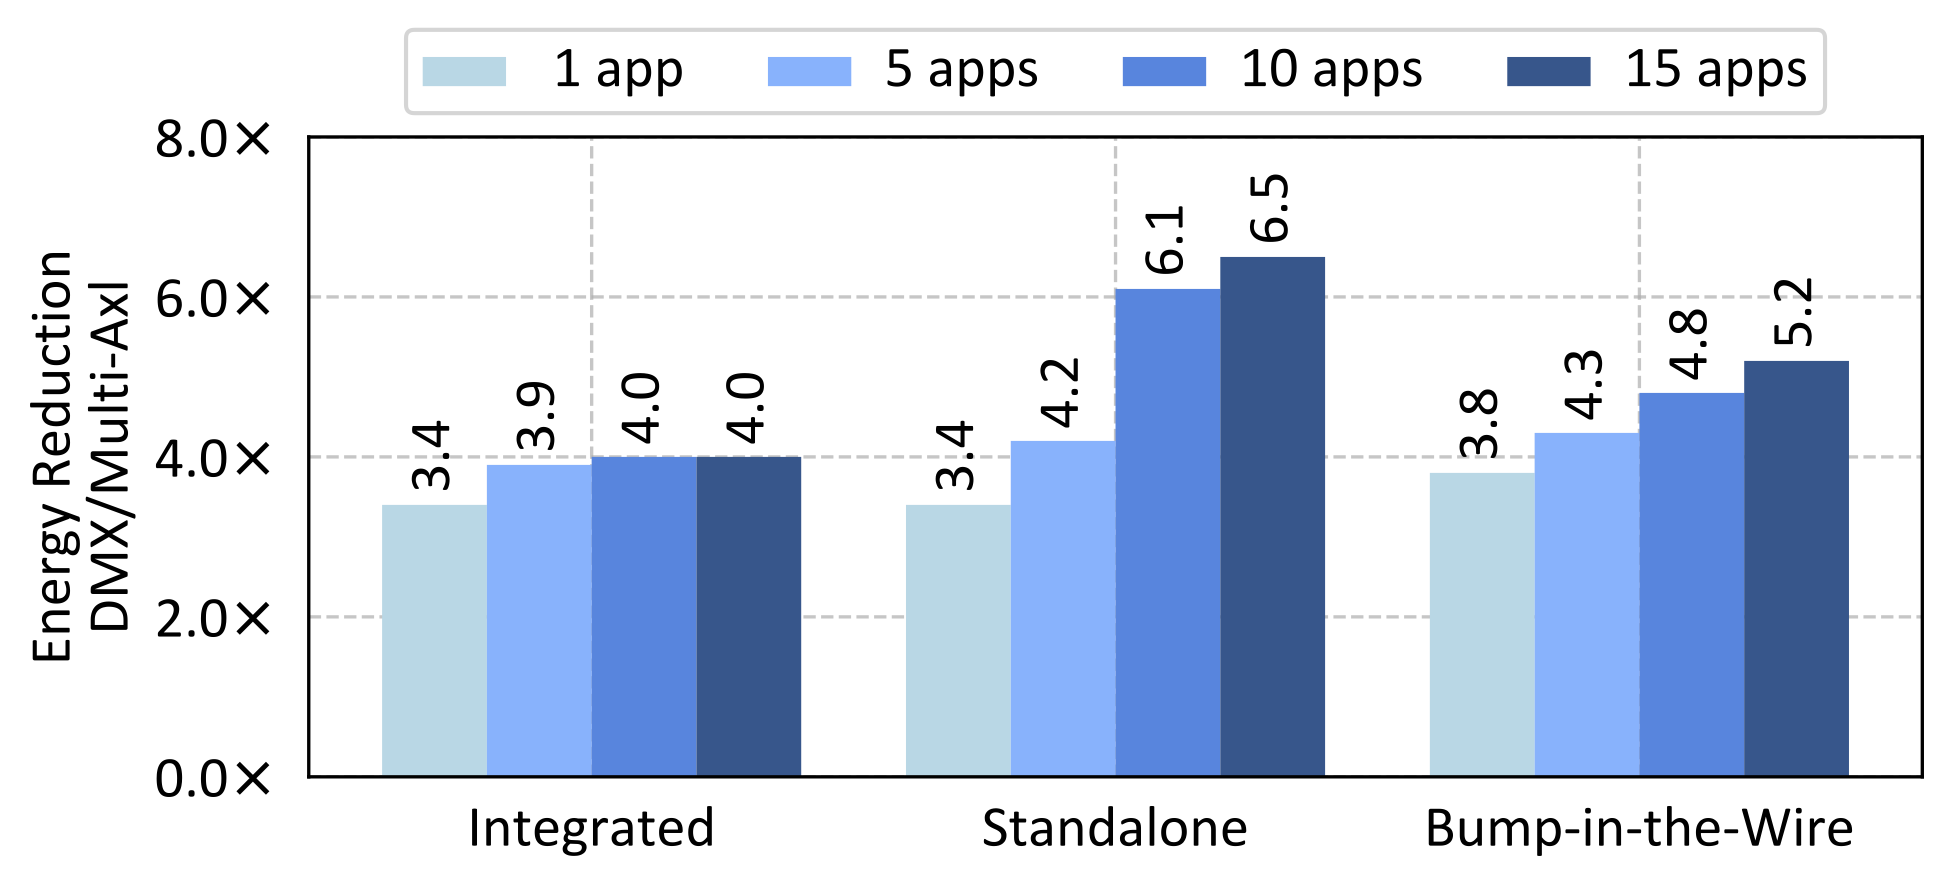
\includegraphics[width=\linewidth]{figure/fianchetto/system-energy-reduction.pdf}
    \caption{System-wide energy reduction, including host CPU cores, accelerators, and \drxs. 
    %
    Bump-in-the-Wire \drx achieves less reduction than Standalone \drx due to its internal PCIe multiplexer shown in Fig.~\ref{fig:drx-config-acc}.
    %
    Integrated, Standalone, and Bump-in-the-Wire \drx draw up to 26\%, 23\% and 28\% more power than the \emph{Multi-Axl} baseline. 
    %
    PCIe-Integrated is not included because we are not able to estimate the power of a \drx-integrated PCIe switch.
    }
    \label{fig:res:energy-drx-placement} 
\end{figure}

\noindent \textbf{Energy reduction with different DRX placements.}
%
Figure~\ref{fig:res:energy-drx-placement} shows system-wide energy reduction provided by different \drx placements compared to \emph{Multi-Axl} baseline.
%
Integrated \drx provides 3.4$\times$, 3.9$\times$, 4.0$\times$, and 4.0$\times$ of energy reduction. 
%
The energy reduction does not scale with the number of concurrent applications because it only benefits from the energy efficiency of the \drx hardware acceleration for data restructuring operations. 
%
Standalone \drx and Bump-in-the-wire \drx provide energy reduction scaling with the increased number of concurrent applications.
%
Bump-in-the-wire \drx placement delivers the best energy reduction of 3.8$\times$ and 4.3$\times$ for 1 and 5 concurrent applications. 
%
Standalone \drx delivers the best energy reduction of 6.1$\times$ and 6.5$\times$ for 10 and 15 concurrent applications because of the reduced bandwidth contention on PCIe links.
%
This is because the extra glue logic and the dual-port PCIe multiplexer are replicated in each Bump-in-the-Wire \drx placement, while such overhead is amortized across the applications on a large Standalone \drx. 
%
PCIe-Integrated is not evaluated for energy reduction because of the difficulty of estimating the energy consumption of a PCIe switch integrated with \drx.
%
\subsection{Sensitivity Studies}
%
\noindent \textbf{Speedup with more than two kernels.}
%
As real-world applications can consist of multiple kernels across domains, it is important for \dmx to scale beyond two kernels. 
%
To evaluate \dmx's scalability with multiple application kernels, 
%
we add a third application kernel to the \pir benchmark, along with its additional data restructuring kernel consisting of reshaping and typecasting. 
%
This third kernel is a Transformer model fine-tuned for Named Entity Recognition (NER). NER identifies personal and sensitive information that is hard to capture for regular expression kernel~\cite{ner-transformer}.
%
We use an open-source BERT implementation for the kernel~\cite{verigoodml:iccad:2021}.
%
% The accelerator takes text as input and performs token embedding lookup on the accelerator like previous BERT implementation on FPGA~\cite{ftrans:ispled:2020}.
%
Figure~\ref{fig:res:multi-kernel}(a) shows the runtime breakdown of this three-kernel benchmark. 
%
Although the benchmark included the compute-intensive NER kernel, the runtime is still dominated by the data restructuring kernels for the \emph{Multi-Axl} baseline.
%
\dmx alleviates the bottleneck of data motion and restores kernel to be the largest contributor that represents 97.2\% to 93.7\% of the end-to-end execution time for one to 15 concurrent applications.  
%
As such, \dmx provides 1.9$\times$ to 4.2$\times$ speedup for one to 15 concurrent applications shown in Figure~\ref{fig:res:multi-kernel}(b).

\begin{figure}[t!]
\begin{subfigure}[ht!]{\columnwidth}
\centering
\includegraphics[width=\columnwidth]{figure/fianchetto/multi-kernel-breakdown.pdf}
\caption{Runtime breakdown}
\label{fig:res:multi-kernel-breakdown}
\end{subfigure}
%
\begin{subfigure}[ht!]{\columnwidth}
\centering
% shifting 
\hspace{-0.75cm}
\includegraphics[width=0.65\columnwidth]{figure/fianchetto/multi-kernel-speedup.pdf}
\caption{Speedup}
\label{fig:res:multi-kernel-speedup}
\end{subfigure}
%
\caption{\dmx reduces data motion overhead to less than 5\% for \pir benchmark extended with Named Entity Recognition kernel.
%\rohan{Shu-Ting when you get some time, please change this color too. Hadi mentioned that he does not like the dark color}
}
\label{fig:res:multi-kernel}
\vspace{-3ex}
\end{figure}

%\revision{
\noindent \textbf{One-to-many and many-to-one data movement.}
%
Cross-domain multi-acceleration of end-to-end applications entails using multiple accelerators.
%
The data movements in multi-acceleration, however, are not necessarily always one-to-one but likely include one-to-many and/or many-to-one data movement between accelerators.
%
Therefore, we want to analyze whether \dmx design can cope with the one-to-many and/or many-to-one data movements in multi-acceleration.
%
To this end, we compare Bump-in-the-Wire \drx against the \emph{Multi-Axl} baseline for one-to-many (i.e., broadcast) and many-to-one (all-reduce) data movement using 4 to 32 accelerators.
%
For broadcast, the baseline first passes the output of the source accelerators to the main memory of the CPU using DMA.
%
%After data restructuring on CPU, the driver clones the restructured data using 8 threads to $N$ DMA buffers and then initiates $N$ DMA transfers to the destination accelerators.
After data restructuring on the CPU, the driver then copies the restructured data and initiates $N$ DMA transfers \emph{sequentially} to the destination accelerators. 
%
All-reduce has two stages: scatter-reduce and all-gather.
%
Both require similar DMA transfers between CPU and accelerators; however, scatter-reduce entails additional steps to first sum the inputs from sources and then scatter the outputs to all destinations. 
%
On the contrary, \dmx's implementation of broadcast and all-reduce utilizes the Bump-in-the-Wire \drx for data restructuring and data movement.
%

Figure~\ref{fig:res:collectives} shows that the \dmx achieves 3.7$\times$ to 5.2$\times$ speedup on broadcast and 5.1$\times$ to 10.5$\times$ speedup for all-reduce on 4 to 32 accelerators.
%
This is because \dmx utilizes \drxs to (1) perform data restructuring and the DMA transfers \emph{in parallel} and (2) eliminate the extra DMA transfers between the accelerators and the CPU.
%
Furthermore, for all-reduce, \dmx uses \drx to accelerate the summation operations.
%
The speedup also scales with the number of accelerators because the amount of data restructuring and data movement scale accordingly to the number of accelerators. 
%
There is a dip when using 16 or more accelerators, but this is due to the additional latency on the PCIe switches that scales with the number of accelerators.
%
\dmx achieved higher speedup in all-reduce compared to broadcast because all-reduce involves more DMA transfers and data restructuring which provided more acceleration opportunity using \drx.
%
% The PCIe switch added to the system when using 16 or more accelerators causes a dip in the relative speedups.
% %
% \dmx achieved higher speedup in All-Reduce compared to broadcast as All-Reduce involves more DMA and memory copy which provided more acceleration opportunity for \dmx.
%
%\dmx's implementation of broadcast and all-reduce avoids PCIe bandwidth contention to the CPU because  Bump-in-the-Wire \drx is local and exclusive to the accelerator.
%
%\dmx also eliminates the extra DMA from accelerators to CPU as well as the memory copy after the data transformation.   
%
%Finally, \dmx uses \drx to accelerate summation operation in the All-Reduce workload.
%
%For inter-accelerator communication, \dmx uses multiple RX/TX data queues on \drx for sending and receiving data from other \drxs as stated in Sec.~\ref{sec:system}.
%
% not this one hanyang. not done yet here.
% \red{This motivates the use of one-to-many and many-to-one data movement between accelerators through \drx in the case of \dmx.} 
%\soroush{why are we doing this experiment? please say that at the beginning}
%Therefore, we compare Bump-in-the-Wire \drx against the \emph{Multi-Axl} baseline for one-to-many (i.e., broadcast) and many-to-one (all-reduce) data movement using 4 to 32 accelerators.
%
%The multi-acceleration baseline orchestrates inter-accelerator operations through CPU and main memory.
%
%For broadcast, the baseline first passes the output of the accelerator to the host CPU's main memory through DMA.
%
%After data transformation, the driver clones the transformed data using 8 threads to $N$ DMA buffers and then initiates $N$ DMA transfers to the destination accelerators. 
%Then, it makes $N$ copy, which $N$ is the number of receiving accelerators, to buffer corresponding to each receiver. The memory copy operation is parallelized by 8 threads. Lastly, it DMAs the $N$ copy to the corresponding accelerator.
%
%For all-reduce, the workflow is similar except it has twice as many memory copies on per-accelerator DMA buffers in the two stages of all-reduce: scatter-reduce and all-gather.
%For all-reduce, the workflow is similar except it has twice amount of memory copy on per-accelerator buffers in the two stages of all-reduce: scatter-reduce and all-gather.
%
% \dmx's implementation of broadcast and all-reduce avoids PCIe bandwidth contention to the CPU because  Bump-in-the-Wire \drx is local and exclusive to the accelerator.
% %
% \dmx also eliminates the extra DMA from accelerators to CPU as well as the memory copy after the data transformation.   
% %
% Finally, \dmx uses \drx to accelerate summation operation in the All-Reduce workload.
% %
%As such, \dmx achieves 3.7$\times$ to 5.2$\times$ speedup on broadcast and 5.1$\times$ to 10.5$\times$ speedup for all-reduce on 4 to 32 accelerators shown in Figure \ref{fig:res:collectives}
%Therefore, \dmx achieves 5.2 $\times$ and 10.4 $\times$ latency improvement on 32 accelerators for broadcast and all-reduce respectively.
%\malian{why doing a simple summation results in such a huge gap in the relative speedup?}
%
%\revision{
%
%The overall improvement scale with the number of accelerators because the amount of data movement scale accordingly to the number of accelerators. 
%
%The PCIe switch added to the system when using 16 or more accelerators causes a dip in the relative speedups.
%
%\dmx achieved higher speedup in All-Reduce compared to broadcast as All-Reduce involves more DMA and memory copy which provided more acceleration opportunity for \dmx.
%

\begin{figure}[t!]
    \centering
    %\includegraphics[width=0.8\columnwidth, cframe=blue!5!blue 0.5mm]
    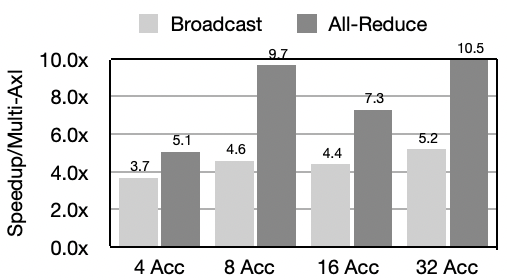
\includegraphics[width=\columnwidth]{figure/fianchetto/collectives.pdf}
    \caption{\dmx eliminates redundant DMA transfers and performs DMA in parallel for broadcast and all-reduce on multi-accelerator setup.}
    \label{fig:res:collectives}
\end{figure}

% \begin{figure}[t!]
%     \centering
%     \includegraphics[width=\columnwidth]{ASPLOS23/figures-resubmit/standalone-underprovision.pdf}
%     \caption{End-to-end latency speedup of different provision levels of Standalone \drx. 
%     Over-provisioning \drx is better in terms of performance and energy consumption because under-provisioning \drx yields lower speedup and uses 1.2$\times$ to 1.4$\times$ more energy.
%     }
%     \label{fig:res:stnadalone-underprovision}
% \end{figure}

% \noindent \textbf{Provision levels of standalone \drx.}
% %
% While deploying end-to-end applications as a service, the Total-Cost-of-Ownership (TCO) is critical to the system design~\cite{e3:atc:2019}.
% %
% The provision levels of Standalone \drx are important as lower levels of provisioning provide lower purchase prices and operating costs.
% %
% Therefore, lowering the provision levels of \drx may be a luring choice when only a few applications are running.
% %
% However, it is important to note that we must make sure that the latency of the end-to-end application stays within the margin.
% %
% To this end, we analyze the impact of different provision levels of \drx.
% %
% The over-provisioned configuration of Standalone \drx provisions just one more Standalone \drx than its need of data restructuring computation.
% %
% The under-provisioned configuration, on the other hand, provisions one less Standalone \drx it needs. The two provision levels do not match the demand for data restructuring but are close to the right-sized provision.
% %
% Over-provisioned Standalone \drx leads to utilization on various levels: 25\%, 62.5\%, 83.3\%, and 93.8\% for 1, 5, 10, and 15 concurrent applications, respectively.
% %
% Under-provisioned Standalone \drx does provide full utilization but it also leads to 16.6\% and 21.6\% lower speedup than the over-provisioned counterpart for 10 and 15 concurrent applications.
% %
% The lower speedup of under-provisioned Standalone \drx is due to increased contention on bandwidth to access \drx.
% %
% This also results in 1.2$\times$ to 1.4$\times$ more energy consumption than its over-provisioned counterpart, though it uses a fewer number of PCIe switches and Standalone \drx.
% %
% Overall, over-provisioning \drx is better in terms of performance and energy consumption.  
%
% \hanyang{I think this is not a well thought-out experiment in general. First, how do you even define under-provision? you can have 1 DRX for 15 applications or 3 DRXs for 15 applications and both of those could still be under-provisioned for the use case, so which result should you report in this case? Generalizing it under one category feels like an over-simplification. Second, CPU-Integrated DRX could also be facing contention, it is not clear what exactly is the problem under study here, what exactly is causing the slowdown in this experiment? I think it is even a little bit trivial since of course you are gonna have some kind of contention when you over-utilize the DRX. My opinion is to delete this section altogether}


%\begin{comment}

\begin{figure}[t!]
    \centering
    \includegraphics[width=\linewidth]{figure/fianchetto/sensitivity-simd-lanes.pdf}
    \caption{Data restructuring latency speedup with different numbers of RE lanes on \drx. The increase of speedup
    is limited after 128 lanes. which is our default configuration.}
    \label{fig:res:simd-lanes}
\end{figure}

\begin{figure}[t!]
    \centering
    %\includegraphics[width=1\columnwidth, cframe=red!5!red 0.5mm]{ASPLOS23/figures-resubmit/drx-acc-arch.pdf}
    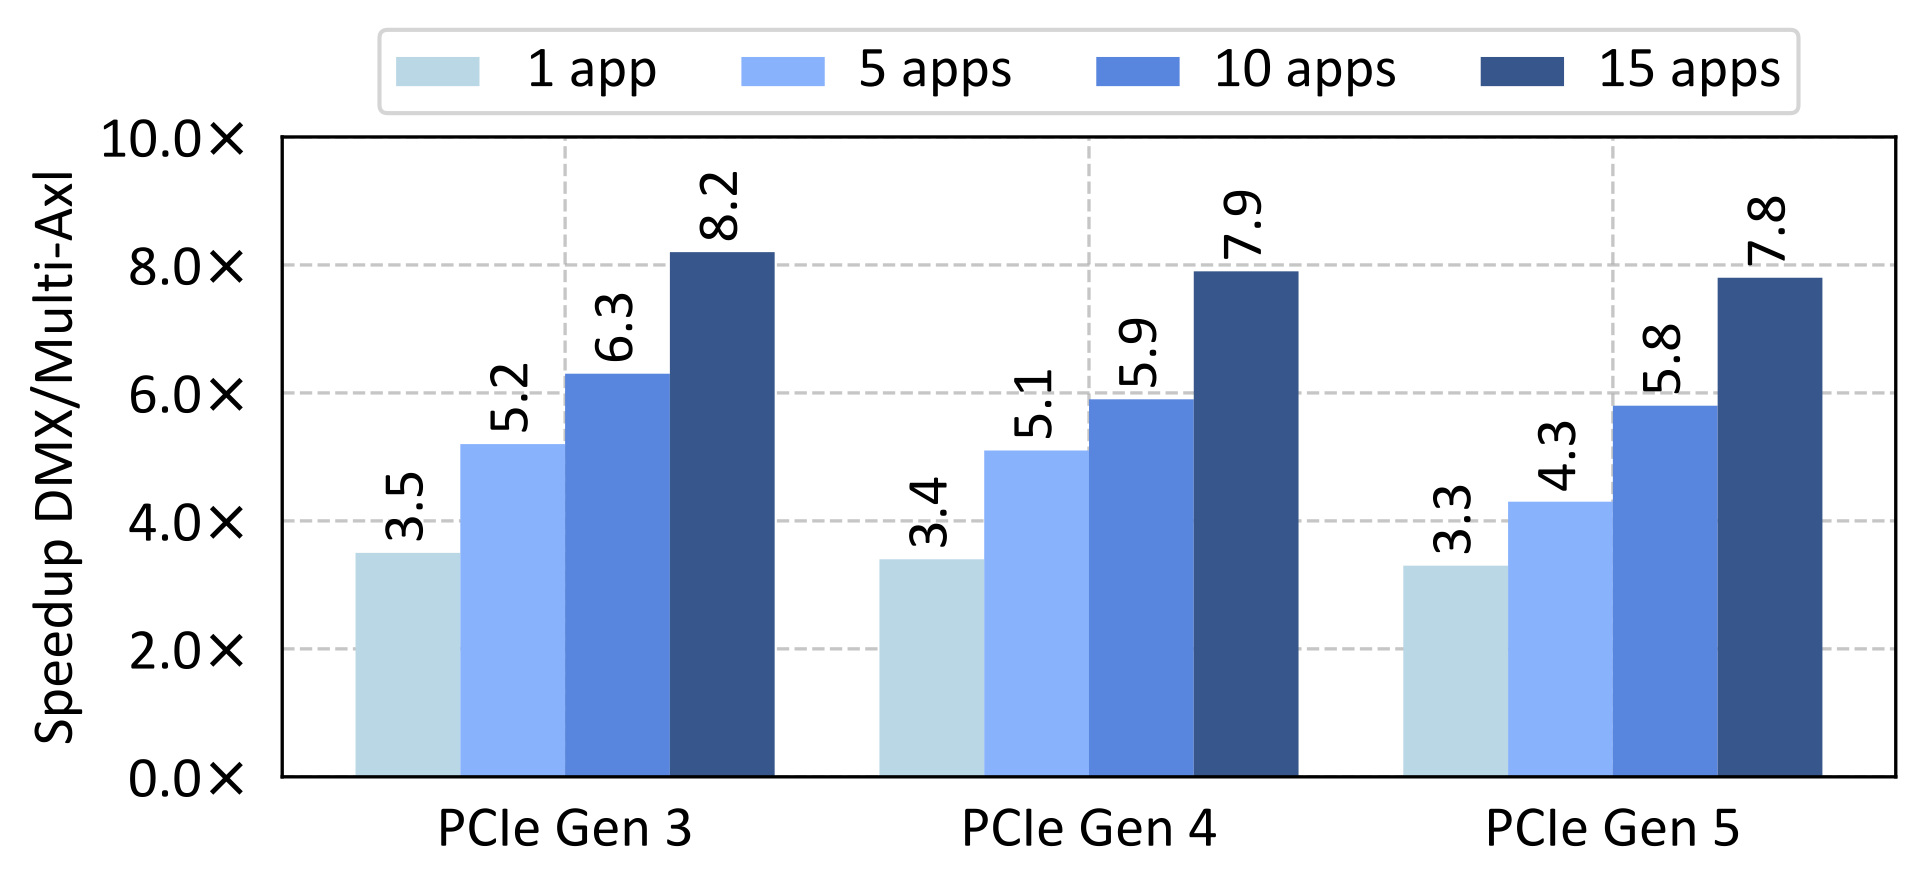
\includegraphics[width=0.98\columnwidth]{figure/fianchetto/speedup-diff-pcie-gens.pdf}
    \caption{\dmx speedup across generations of PCIe. PCIe Gen4 and Gen5 result in a slight decrease of speedup because their corresponding \emph{Multi-Axl} baselines improve more than their \dmx counterparts.}
    \label{fig:res:pcie-gens}
\end{figure}


\noindent \textbf{DRX hardware configurations.}
\label{sec:results:hardware-config}
%
To understand the sensitivity of \dmx to the amount of compute resources in \drx, we sweep the number of RE lanes for \drx and compare its performance to the \emph{Multi-Axl} baseline that performs data restructuring on CPU. 
%\soroush{why 16? is it different fron the baseline config that we used to show the speedup numbers? if yes, why?}.
%
% The default configurations used throughout the experiments are 128 vector lanes and 64KB of data scratchpad.
% %
%\noindent \textbf{Sensitivity Analysis: SIMD lanes.}
Figure~\ref{fig:res:simd-lanes} shows the speedup achieved for the different number of lanes for \drx: from 32 to 256. 
%
The speedup improves with the number of lanes increasing up to 128 lanes by taking advantage of available data parallelism in data restructuring operations.
%
%\rohan{from the figure, it does not seem like the speedup saturates}
%
However, the increase of speedup of \drx is limited after 128 RE lanes, and increasing the lanes to 256 does not provide noticeable benefits.
%
Therefore, we use 128 RE lanes as the default configuration for \drx throughout the experiments. 
%as the optimal point for performance.
%\end{comment}


\noindent \textbf{Different PCIe generations.}
Newer PCIe generation provides significantly more bandwidth and the increased bandwidth can potentially negate the performance benefit of \dmx. 
%
To understand the impact of different generations of PCIe, we compare the Bump-in-the-Wire DRX latency speedup on PCIe Gen 3 with PCIe Gen 4 and Gen 5.
%
Figure \ref{fig:res:pcie-gens} shows that using PCIe Gen 4 and Gen 5 resulted in a slight decrease of speedup because their corresponding \emph{Multi-Axl} baselines improve more than their \dmx counterparts.
%
Across PCIe generations, the baselines and \dmx show different levels of improvement only in data movement latency. 
%
Such differences come from the following two reasons.
%
First, the baselines face more bandwidth contention than the \dmx and thus benefit more from the increased PCIe bandwidth per lane.
%
Second, the baselines are able to use more PCIe lanes to reduce bandwidth contention from accelerators to CPUs with PCIe Gen 4 and Gen 5 compared to CPUs with PCIe Gen 3~\cite{intel-cascade-lake, intel-ice-lake, intel-sapphire-rapids}. The results shown in Figure~\ref{fig:res:pcie-gens} suggests that the bottleneck of \emph{Multi-Axl} configuration is not just the PCIe interconnect, but also the data restructuring computation. 

%\begin{comment}
% \begin{figure}[ht]
%     \centering
%     \includegraphics[width=\columnwidth]{figure/fianchetto/cxl-cpu-solutions.pdf}
%     \caption{CXL shows negligible slowdown on the multi-acceleration baseline over PCIe. Integrated \drx which integrates \drx on CPU shows similar speedup on PCIe and CXL.}
%     \label{fig:res:cxl-cpu-solutions}
%     \vspace{-2ex}
% \end{figure}
%
% \noindent \textbf{CXL as Interconnect Alternative.}
% %\subsection{Interconnect Alternative: CXL}
% %\label{sec:results:cxl}
% %\stingw{again, why on earth do we want to do this? we can say this reduce the control overhead, e.g. interrupts and scheduling. CXL translate that to a cache coherency problem.}
% % CXL~\cite{cxl-3-0-spec} is an interconnect alternative that can reduce the control overhead, such as interrupts, for multi-acceleration systems. CXL translates the overhead of the non-coherent DMA approach to cache coherency overhead.
% CXL~\cite{cxl-3-0-spec} is an interconnect alternative that can reduce the control overhead, such as interrupts, for multi-acceleration systems with attached expandable coherent memory systems. CXL trades off the overheads of the non-coherent DMA approach with overheads for supporting cache coherency.
% %
% Both multi-acceleration and Integrated \drx with CXL shows no improvement and a negligible slowdown in Fig.~\ref{fig:res:cxl-cpu-solutions}. 
% %
% The accelerators in our benchmarks are fed with input data between 6$\sim$16 MBs as they do not operate on the granularity of a cache line. Therefore, CXL provides no tangible benefit to our benchmarks running with \dmx.
% %
% This observation is consistent with prior work~\cite{cxl-model:exhet:2022} modeling CXL which is calibrated with GPU and FPGA measurements. They observed CXL outperforming PCIe only for transfers less than 12.7 KB and with frequent host-accelerator interactions. 

% The energy efficiency of \drx is the primary reason for energy reduction shown for a single application as
% \drx consumes less power and performs data restructuring operations more efficiently than CPU. 
% %
% Integrated \drx draws more energy than the other two placement strategies.
% %
% Integrated \drx runs longer as shown in its less latency speedup in Fig.~\ref{fig:res:speedup-drx-placement}. This keeps PCIe switches and \drx active for a longer period of time and results in the worst energy reduction among the three.
% %
% Standalone \drx consumes less energy than Integrated \drx because of its better speedup. 
%\end{comment}


% \vspace{-1ex}
\section{Related Work}
\label{sec:related}
%
Real-world applications span multiple domains, posing a challenge for end-to-end acceleration.
%
While the research community has explored accelerators across diverse domains~\cite{q100:asplos:2014, meet-the-walkers:isca:2013, doppiodb:fpl:2017,chiosa:pvldb:2022, acc-yolov3:iscas:2020, wfa:fpl:2021, genstore:asplos:2022, segram:isca:2022, meet-the-walker:micro:2013,murray:micro:2016,robox:isca:2018,pointacc:micro:2021,robomorphic:asplos:2021}, the adoption of these heterogeneous accelerator to accelerate a single end-to-end application is challenging.
%
The challenge arises due to the diverse data formats generated and consumed by each accelerator.
%
This necessitates restructuring inputs and outputs across accelerators. 
%
While some prior works have focused on performed data restructuring using CPUs, \dmx introduces the concept of data motion acceleration of for efficient cross-domain multi-acceleration with heterogeneous DSAs.
%
We review the most relevant related work in three areas: data movement, data restructuring, and interconnect fabrics integration below.
%

\noindent \textbf{Data movement.}
%
Prior works studied point-to-point data movement between GPUs~\cite{gpudirect:2019}, between GPU and storage~\cite{morpheus:isca:2016,spin:atc:2017,nds:micro:2021}, between NIC and accelerator~\cite{p2pdma:apsys:2020,lynx:asplos:2020,flexdriver:asplos:2022}, and between on-chip accelerators~\cite{arc:dac:2012}. 
%
Prior works have used various techniques such as scheduling~\cite{wisefuse:sigmetrics:2022, mahapatra:mlarchsys:2022, paragon:asplos:2013, lynx:asplos:2020,flexdriver:asplos:2022} to co-locate multiple domains on the same system. 
%
While these works only optimize the data movement, non-trivial operations of the data restructuring still consumes a significant fraction of the data motion.
%
Intel Data Stream Accelerator~\cite{intel-dsa} and DCS~\cite{dcs:micro:2015, dcs-ctrl:isca:2018} share a similar insight, both lack programmability and hence have limited capacity to optimize data restructuring.
%
This work in contrast leverages \drxs as a compute-enabled glue that links different heterogeneous accelerators together and makes them appear as a monolithic but composable accelerator for the application.
%

\noindent \textbf{Data restructuring.}
%
For message serialization, Optimus Prime~\cite{optimusprime:asplos:2020} and Protobuf accelerator~\cite{protobuf:isca:2021} design an accelerator for RPC message serialization.
%
HGum~\cite{hgum:reconfig:2017} and Fletcher~\cite{peltenburg-2019-fletcher} implement serialization on FPGAs for acceleration.
%
For machine learning pipelines, tf.data~\cite{tf.data:pvldb:2021}, DSI~\cite{dsi-dlrm:isca:2022}, DALI~\cite{nvidia-dali:2018} optimize data restructuring on GPU with programmable operations.
%
In contrast to these prior works that only optimize data restructuring for a single accelerator, this chapter investigates data restructuring and movement for multi-acceleration with heterogeneous devices.
%

\noindent \textbf{Interconnect fabrics.}
%
Previous works have used PCIe's Non-Transparent Bridge (NTB) to enable PCIe to support multiple hosts with more than one root complex, which performs address translation for operations in a specific memory range~\cite{hou:hpca:2013,smartio:tocs:2021}.
%
Point-to-point DMA over PCIe fabric is enabled by a shared address space across all devices~\cite{gigaio-pcie-swtich}.
%
CXL 3.0 or later allows accelerators on different servers to be connected seamlessly by using fabric switching to link racks of devices and accelerators~\cite{cxl-3-0-spec}.    
%
DUA~\cite{dua:nsdi:2019} creates an overlay fabric on top of the existing physical communication stacks, such as PCIe, Ethernet, DDR, etc.
%
These works can connect accelerators without addressing data restructuring for multi-acceleration.
%
This work, however, tackles data motion challenges to maximize the performance of multi-acceleration.

\section{Conclusion}
\label{sec:conclusion}
%
% With heterogeneous data centers, while accelerators are becoming a prominent component, there is a need for considering issues that arise in the intersection of system and architecture.
In this chapter, we quantified the data motion performance and cost of chaining heterogeneous domain-specific accelerators for multi-acceleration.
%
The results showed that the data motion overhead curtails the end-to-end speedup of accelerating each domain on a set of heterogeneous accelerators. 
%
The chapter introduced \dmx that seamlessly weaves together multiple accelerators that deliver the performance of a large, monolithic cross-domain accelerator. 
%
On average, \dmx provides between 3.4$\times$ to 8.2$\times$ speedup, 3.0$\times$ to 13.6$\times$ higher throughput, and 3.8$\times$ to 5.2$\times$ energy reduction.

Even with current single-domain accelerators, overheads of moving data on- and off-chip is presently a dominant factor that limits the performance and energy efficiency of gains~\cite{horowitz:isscc:2014, accelerator-cluster:hoti:2023}. 
%
The impact of the data motion--highlighted in this chapter--will worsen when cross-domain accelerators are chained in future datacenters to cater to the requirements of emerging end-to-end applications.
%
This even includes the multimodal generative AI applications that use multiple models and require acceleration beyond neural networks (e.g., vector database lookups, search, etc.).
%
Heterogeneous/3D integration coupled with emerging high-bandwidth chiplet-to-chiplet interconnects such as UCIe can improve data movement, but not data restructuring that requires computation.
%
As such, embedding our \dmx concept and architecture within these interconnects can synergistically unlock the the potential of cross-domain multi-acceleration for next-generation dataceneters.

\section{Sources for Material Presented in This Chapter}
%
Chapter~\ref{fianchetto:chap}, in part, reprints material as it appears in a paper titled: "Data Motion Acceleration: Chaining Cross-Domain Multi Accelerators"
by Shu-Ting Wang, Hanyang Xu, Amin Mamandipoor, Rohan Mahapatra, Byung Hoon Ahn, 
Soroush Ghodrati, Krishnan Kailas, Mohammad Alian, and Hadi Esmaeilzadeh~\cite{dmx:hpca:2024}.
% 
The dissertation author was the primary researcher and author of this material.